\setchapterpreamble[u]{\margintoc}
\chapter{Optimization of LiDAR scans}
\labch{lidar_optimization}
\label{sec:lidar_optimization}

\section*{About this chapter}

\marginnote[13.0cm]{Although this optimization provides a minimum number of optimal scan positions, these are still required to be performed by humans. Therefore, positions must be optimized but also narrowed to make this task less time-consuming.}
This chapter presents a pipeline for optimizing \acrshort{tls} scans in indoor environments using the previously implemented \acrshort{lidar} simulation. To solve this problem, metaheuristics such as local search (\acrshort{ls}), tabu search and genetic algorithms (\acrshort{ga}) operate over a set of positions, whose fitness is measured after their synthetic \acrshort{lidar} point cloud. The expected outcome is a set of optimal locations that help to scan a real-world scenario by ensuring proper density, coverage and quality. In comparison with previous research, buildings are represented by 3D models, thus enabling to account for sensors with adaptive height. The literature of Planning 4 Scanning (\acrshort{p4s}) has utilized four metrics to evaluate plannings: \acrshort{loa} (accuracy), \acrshort{lod} (detail), \acrshort{loo} (overlap) and \acrshort{loc} (coverage). This work comprises the previous four metrics into three functions that reduce the number of steps in this multi-objective optimization. Following the approach of Chapter \ref{sec:lidar_simulation}, the \acrshort{lidar} scans as well as part of the optimizations were implemented in the \acrshort{gpu} or as multi-core \acrshort{cpu}. Rather than selecting among different metaheuristic algorithms, these will be chained to narrow the search space. For instance, \acrshort{ls} helps to provide a rapid improvement of initial positions, whereas \acrshort{ga} narrows this search space by generating a solution that encodes which positions ought to be used without worsening the metrics. That is, \textbf{which is the minimum number of points (and which points) required to solve the optimization while still guaranteeing some minimal requirements?} This problem has been previously referred to as the NP-complete set-coverage problem \cite{li_probability_2021, mohamadi_efficient_2021, roostapour_pareto_2022} if the number of solutions, $n$, is known. However, this case study is even more cumbersome since the number of required solutions is not known unless defined by the end user. 

\begin{kaobox}[frametitle=Case study of \acrshort{tls} optimization: Building Information Modelling]
\acrshort{tls} scans are very time-consuming as they are operated by humans whose labour is to place the \acrshort{lidar} sensor on a limited number of locations that may contribute, with better or worse results, to generate a composite point cloud. However, temporal repeatability must be guaranteed in some environments, thus requiring deterministic planning. A case study where these requirements are easier to understand is on the monitoring of buildings in the construction industry. Periodic scans help to track the conditions of a building, which can be saved in a Building Information Modeling (\acrshort{bim}) \cite{macher_point_2017}. This data representation encodes the features of a building, including 3D design drawings, materials, costs and safety specifications, and provides an interface for the management of 4D applications. Together with \acrshort{tls}, it enables the monitoring of continuously evolving buildings to preserve cultural heritage, track its current state and maintain repair records \cite{rocha_scan--bim_2020, andriasyan_point_2020, moyano_bringing_2020, ham_phased_2020}. However, monitoring buildings over time is time-consuming, especially in dynamic environments. Also, \acrshort{tls} scans are given by multiple point clouds that must be later fused, and for this task, there must be some notable overlapping among them, or at least allow us to distinguish visible markers \cite{gollob_comparison_2020}. In this case study, the development of tools for planning \acrshort{tls} surveys plays a key role. 
\end{kaobox}

The main contribution of this work is the implementation of a massively parallel optimization solver using smooth objective functions to measure the fitness of individual solutions, instead of being supervised by thresholds as in previous work. Starting solutions are locally enhanced; otherwise, a huge number of grid partitions with a large memory footprint are required. Then, the optimal subset of locations is estimated with genetic algorithms (\acrshort{ga}), with an objective function that implicitly narrows the number of scans. The outcome of \acrshort{ga} is further refined to guarantee the overlapping of individual scans using a Greedy approach. The input models used during the experimentation are large \acrshort{cad} scenarios from \acrshort{bim} projects authored by Autodesk Revit\textsuperscript{\textregistered}. As a result, this work is able to provide a near-optimal set of locations aimed at optimizing the monitoring of buildings. Furthermore, these optimizations are performed using a parameterized \acrshort{lidar} that can be adjusted according to the specifications of commercial sensors. 

\section{On the optimization of TLS scans}

3D imaging technology is widespread in the construction industry for tracking building progress. It enables capturing the environment geometry in a precise and highly detailed way. Rather than collecting their geometry as polygonal meshes, these are scanned to generate 3D point clouds. In this regard, \acrshort{tls} has been increasingly being used to collect large datasets from buildings \cite{shariq_revolutionising_2020} and cultural heritage remains \cite{banfi_integration_2019, ham_phased_2020, andriasyan_point_2020}, among others. Some of the main shortcomings of \acrshort{tls} technology are the occlusion and range limitations \cite{soudarissanane_optimizing_2012}. Hence, planning \acrshort{tls} scans may help to mitigate this by 1) minimizing the number of scans, 2) generating a point cloud with uniform density, and 3) reducing the occlusion from scene objects. All these three objectives are equally affected by the location and configuration of the scanner. Other \acrshort{lidar} technologies have arisen as suitable alternatives to \acrshort{tls} for addressing the aforementioned drawbacks. However, these are still recent, and despite solving some of these drawbacks, others arise. For instance, \acrshort{lidar}s mounted on backpacks reduce the acquisition time and cover large areas \cite{rodriguez-gonzalvez_mobile_2017}, but the path should be carefully planned to avoid occlusion and guarantee coverage. Also, their point density is lower \cite{bienert_comparison_2018}.

Regarding the optimization of \acrshort{tls} scans in buildings, this field of research is frequently referred to as Planning for Scanning (\acrshort{p4s}). Most of the studies narrow 3D environments to 2D cross-sections, or simplify the scene primitives into others whose collisions are easier to solve, even wrapping a set of primitives (e.g., voxelizations \cite{wakisaka_optimal_2019}). Also, it often requires previous knowledge of the scenario. For instance, \acrshort{oobb}s have been utilized over environments in which \acrshort{aabb}s did not fit well to rotated, non-planar surfaces \cite{li_3d_2022}. On the other hand, \acrshort{dsm}s have also been explored in 2.5D optimizations \cite{starek_viewshed_2020}. However, most of these works are based on the iterative find of the Next Best View (\acrshort{nbv}), while others apply heuristics such as Greedy \cite{ giorgini_sensor-based_2019}, \acrshort{sa} \cite{chen_indoor_2018}, \acrshort{ga} \cite{jia_comparison_2017}, Particle Swarm Optimization (\acrshort{pso}) \cite{jia_comparison_2017} and Integer Programming \cite{wakisaka_optimal_2019}.

The main drawbacks found in previous \acrshort{p4s} work are 1) the widespread use of greedy algorithms to determine optimal plannings, 2) the simplification of input scenarios to speed up solutions, 3) the use of objective functions relying on user-defined thresholds (range, angle, etc.) and 4) the lack of massively parallel algorithms that help in reducing the latency. 

\section{Synthetic scenarios}

Input scenarios are triangle meshes depicting buildings with one or multiple levels, extracted from publicly available \acrshort{bim} projects. These are not constrained to any standard, and therefore, the number and size of the polygons vary. Typically, polygons in walls, floor and ceiling surfaces are larger than those used to represent furniture. However, \acrshort{tls} scans must reach as many polygons as possible. Consequently, operating with surfaces of similar dimensions would greatly benefit a non-weighted planning algorithm. To this end, triangle meshes can be subdivided to reach a nearly uniform triangle size. Note that it is hard to achieve since items such as furniture have a high \acrshort{lod} that cannot be reached by other items, at least not without a large memory footprint. From here, the best choice is to recursively subdivide polygons until their area is below a threshold. Following, scenarios are indexed in a \acrshort{bvh} to be rapidly traversed.

\begin{marginfigure}[-5.0cm]
    \centering
    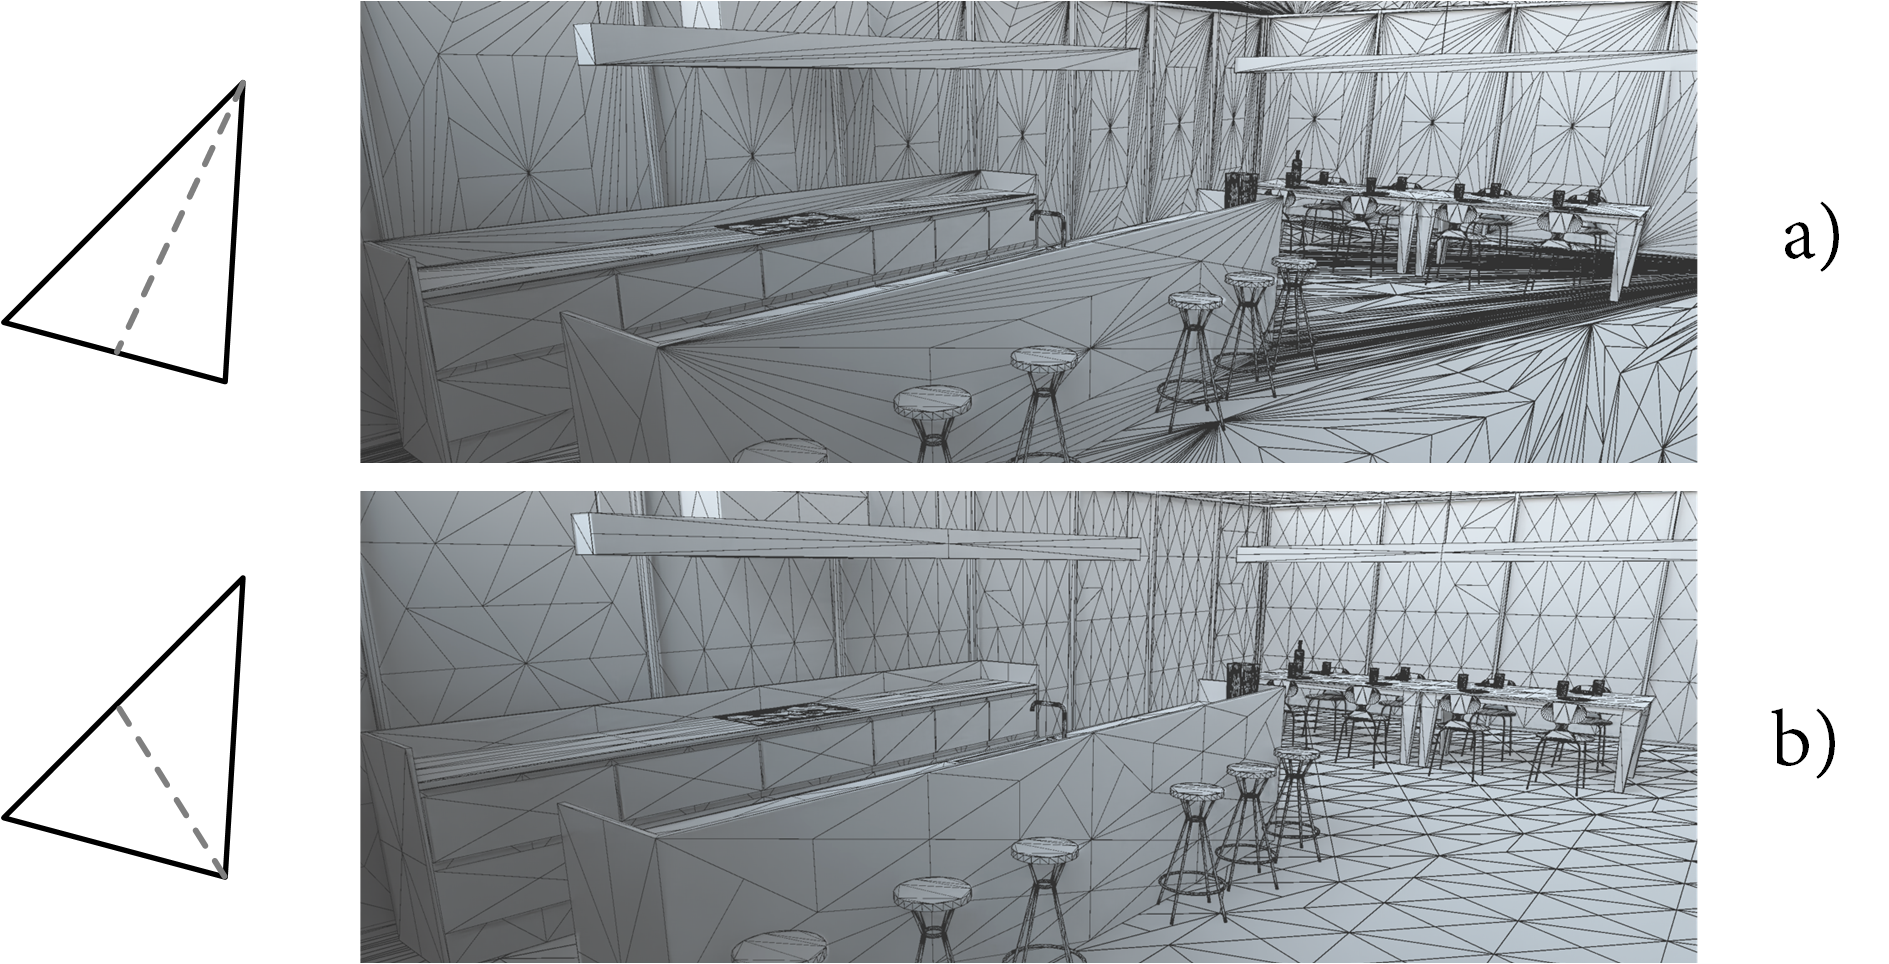
\includegraphics[width=\linewidth]{figs/lidar_optimization/triangle_subdivision.png}
	\caption{Two different triangle subdivisions over the same scene. a) Triangles subdivided by iterating through the edge to be split, and b) triangles subdivided with the proposed method.}
	\label{fig:triangle_subdivision}
\end{marginfigure}
Several approaches are effective to subdivide polygons, although some of them yield aesthetic results (see Figure \ref{fig:triangle_subdivision}). Whether the edge to be split is selected randomly, the triangle can be subdivided into large triangles that degenerate into segment-like polygons. This hardens the detection of collisions in later ray-triangle intersections, together with the loss of precision from using floating point data. Instead, the longest edge within each triangle can be split, thereby generating triangles with a uniform edge length.

\section{Solution encoding}

\begin{marginfigure}[-2.0cm]
    \centering
    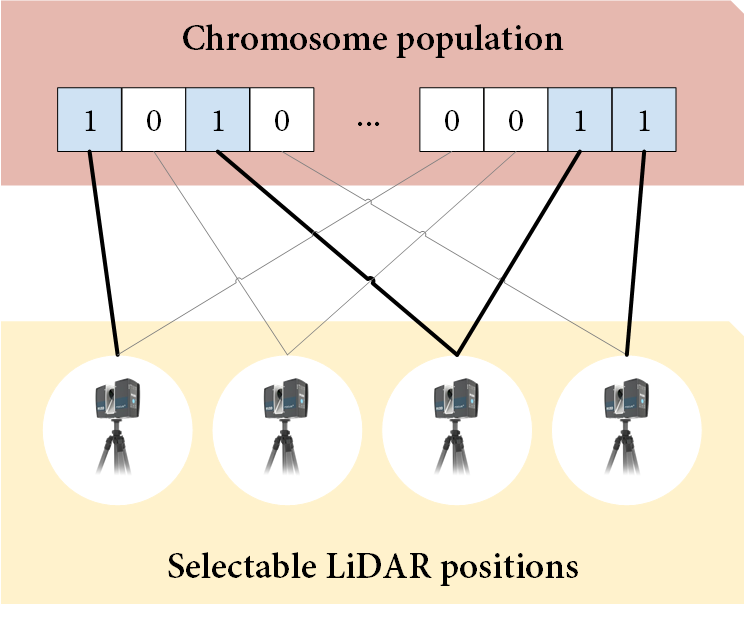
\includegraphics[width=\linewidth]{figs/lidar_optimization/solution_encoding.png}
	\caption{Binary encoding of active \acrshort{lidar} solutions for a genetic algorithm.}
	\label{fig:solution_encoding}
\end{marginfigure}
Candidate solutions in \acrshort{ga} are encoded as a buffer of binary values indicating which minimal set of \acrshort{lidar} positions will be used for scanning. Each binary value is defined as an activation indicating whether this location will be used or not in the final planning. Firstly, positions are either uniformly or randomly sampled along the selected building level. Then, these are optimized with small changes whose impact will be measured by means of multiple metrics. Finally, \acrshort{ga}s are intended to minimize the number of \acrshort{tls} scans while maximizing the coverage of a \acrshort{lidar} point cloud.

With this sequence in mind, initial solutions are stored as $xyz$ coordinates, whereas the solutions of \acrshort{ga} are encoded as vectors of binary values $[b_0, b_1, b_2, ..., b_{k-1}]$, where $b_i \in \{0, 1\}$ and $k$ is the number of solutions generated on the previous spatial search. Although activating $k$ solutions provide the most complete scan, the \acrshort{ga} is intended to minimize the time required by human operators for scanning. Figure \ref{fig:solution_encoding} shows the proposed solution encoding for \acrshort{ga}s. Binary values can be represented by Boolean data in the \acrshort{cpu}; however, this data type is not uniformly represented in \acrshort{cpu} and \acrshort{gpu} hardware. Instead, Boolean values can be expressed using a minimal integer encoding in the \acrshort{gpu} hardware with the \verb|uint8_t| data type. In the \acrshort{gpu}, it requires using the recent \acrshort{glsl}'s \verb|GL_NV_gpu_shader5| extension. Representations with a lower memory footprint are indeed possible with bit-level encoding, at the expense of more intricate operations in accesses and modifications. Nevertheless, the experiments that are later presented allocate a few \verb|MBs| at most.

\section{Metrics}

Fitness functions evaluate the quality of candidate solutions to help in their optimization and determine which are the best candidates. In this section, a solution is represented as a set of $n$ different scans in the same building level, which are evaluated using four metrics. First, the number of scanned polygons provides a trivial measure of the coverage of the scenario ($F_1$: \acrshort{loc}). Also, the uniformity of the scanned points in polygons helps to account for  \acrshort{lod}, \acrshort{loa} and \acrshort{loc} ($F_2$). Finally, \acrshort{tls} scans require a minimum overlapping factor among them to guarantee that they can be later fused in post-processing ($F_3$: \acrshort{loo}). 

\subsection{Level of accuracy, coverage and resolution}

The \acrshort{loc} metric is trivially solved by calculating the number of scanned polygons. However, measuring the uniformity of a point cloud is not as trivial. Instead of providing the required resolution, the optimal value can be computed during pre-processing. Therefore, a nearly optimal resolution is computed polygon-wise by measuring the average distance between uniformly sparsed points. These points were obtained by retrieving two values ($u$ and $v$) from a uniform distribution and used together with the parametric form of a triangle. Therefore, polygons with a mean distance above the reference mean are accordingly penalized on the overall fitness of a planning solution. As a result, point clouds covering a polygon only with a few points within a triangle are heavily penalized (see Figure \ref{fig:f2_metric}). As in previous chapters, \acrshort{qmc} samplers approximate better what is expected from a randomized, yet uniform, scan. 

\begin{figure*}
    \centering
    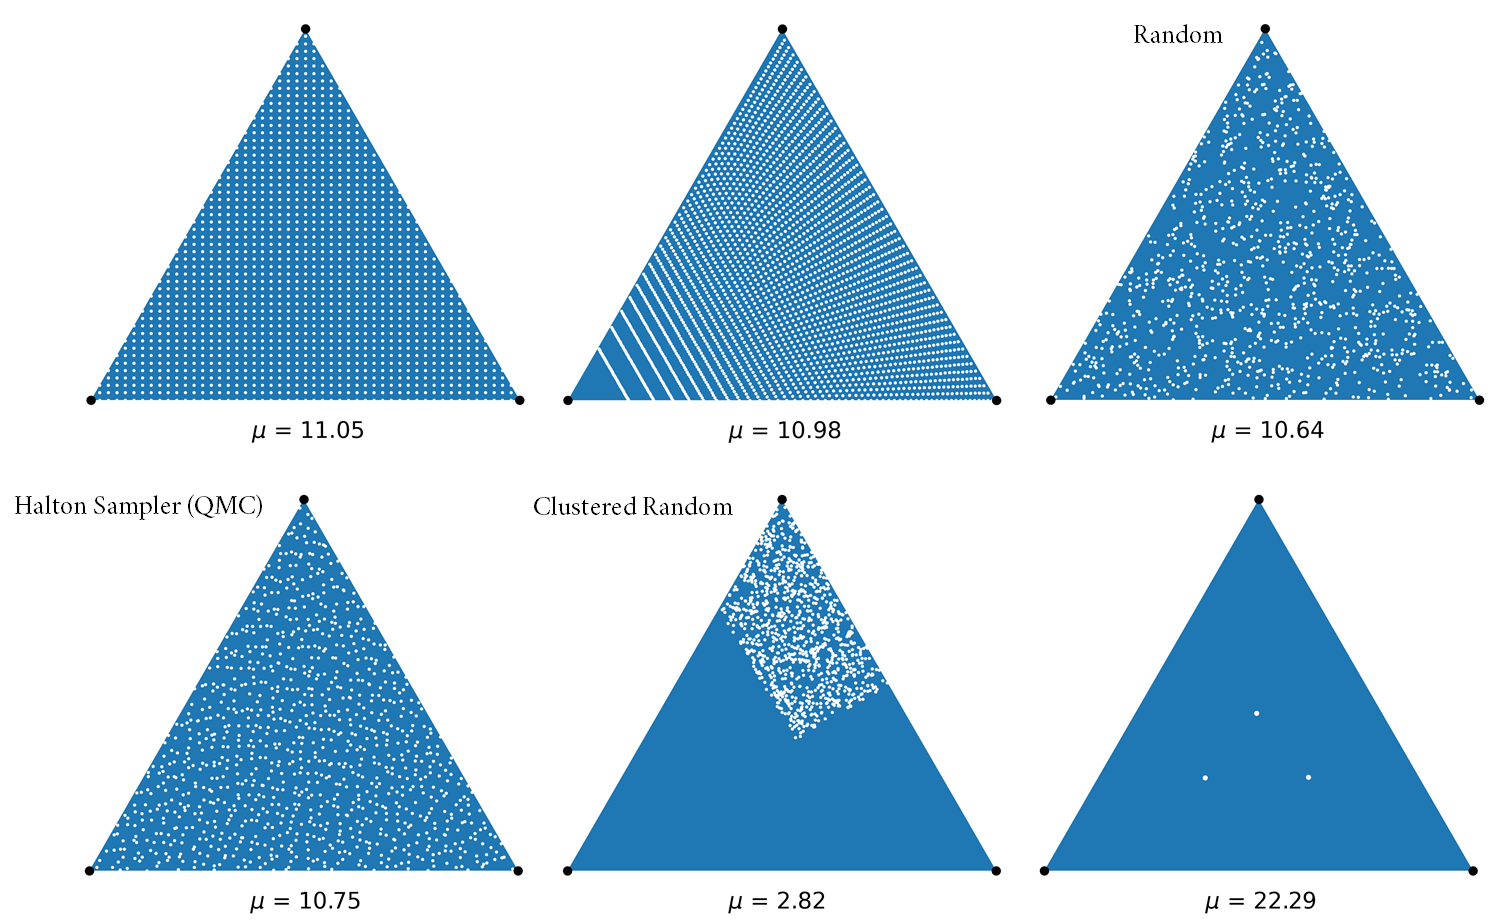
\includegraphics[width=\linewidth]{figs/lidar_optimization/distance_metric.png}
	\caption{Average distance ($\mu$) of every sampled point with the rest. From left to right, and from top to bottom: uniform grid distribution, uniform random sampling of $u$ and $v$, random distribution, \acrshort{qmc} random distribution, random distribution only for a part of the triangle and three points uniformly scattered.}
	\label{fig:f2_metric}
\end{figure*}

$F_1$ and $F_2$ metrics allow enhancing starting positions by translating them towards better locations. They can be either applied to one or multiple locations. In terms of preferences, the point cloud's uniformity and accuracy are typically chosen over coverage for a single scan. Despite this, both $F_1$ and $F_2$ are evaluated during optimization, with $F_1$ working as a secondary metric that helps to untie scenarios where multiple solutions have the same $F_2$ value. $F_1$ and $F_2$ are defined in Equation \ref{eq:metric_count} and \ref{eq:uniformity_error} for evaluating a set of solutions, $K$. Individual solutions have a buffer of collided triangles, $T$, with each one being intersected by a set of points, $P$. The set of collided triangle indices is denoted by $L$, with each index appearing only once. Finally, the whole set of triangles is $S$.
\begin{align*}
    \textit{F}_{1} &= \sum_{s=1}^{\abs{S}} 1[t_s \in \{L_1, L_2, ..., L_k\}]
    \numberthis \label{eq:metric_count}\\
    \textit{F}_{2} &= \sum_{k=1}^{\abs{K}} \left(\sum_{s=1}^{\abs{S}} d_{\textit{optimal}_{s}} - \sum_{l=1}^{\abs{L_k}} d_{\textit{optimal}_{l}}  +\right.\\ & 
    \left. + \sum_{t=1}^{\abs{T_k}} \left(\frac{\sum_{i=1}^{\abs{P_t}} \frac{\sum_{j=1}^{\abs{P_t}} d^{2}(p_i, p_j)}{\max\left(\abs{P_t} - 1, 1\right)} \cdot (2 - \abs{\widehat{n}_{t_{k}} \cdot \widehat{\left(r_{o} - p_{i}\right)}})}{\max\left(\abs{P_t}, 1\right)} - d_{\textit{optimal}_{t}}\right)\right)
    \numberthis \label{eq:uniformity_error}
\end{align*}
where $F_1$ represents the number of different intersected polygons and $F_2$ estimates the accuracy by measuring the distance from the optimal uniformity to the computed one. $d$ represents a distance function, e.g., the Euclidean distance, $t_s$ is a triangle index in $S$, $\hat{n}$ is the normal vector of a triangle, and $r_o$ is the location of the sensor's emitter. Instead of only considering the average dissimilarity from the expected uniformity in intersected primitives, $F_2$ also sums the dissimilarity from the rest of, the non-collided, polygons. However, the summed dissimilarity from intersected polygons must be subtracted to avoid penalizing solutions with a higher number of points (Figure \ref{fig:f2_sampling}). Remark that $F_2$ intends to minimize the measured dissimilarity to the estimated optimal inter-point distance. Therefore, the number of reached polygons, $F_1$, is implicitly considered in this expression by penalizing scans that only reach a small number of polygons.

Also, note the sensor's range is frequently integrated into the \acrshort{loa} metric by discarding returns whose distance is above the maximum allowed distance. However, these criteria can be integrated during the \acrshort{lidar} simulation, rather than worsening the efficiency of $F_2$ estimations. The approach followed considers a distance much lower than the typical range of real-world sensors, thus improving the \acrshort{loa} of the simulated planning.

\begin{figure}
    \centering
    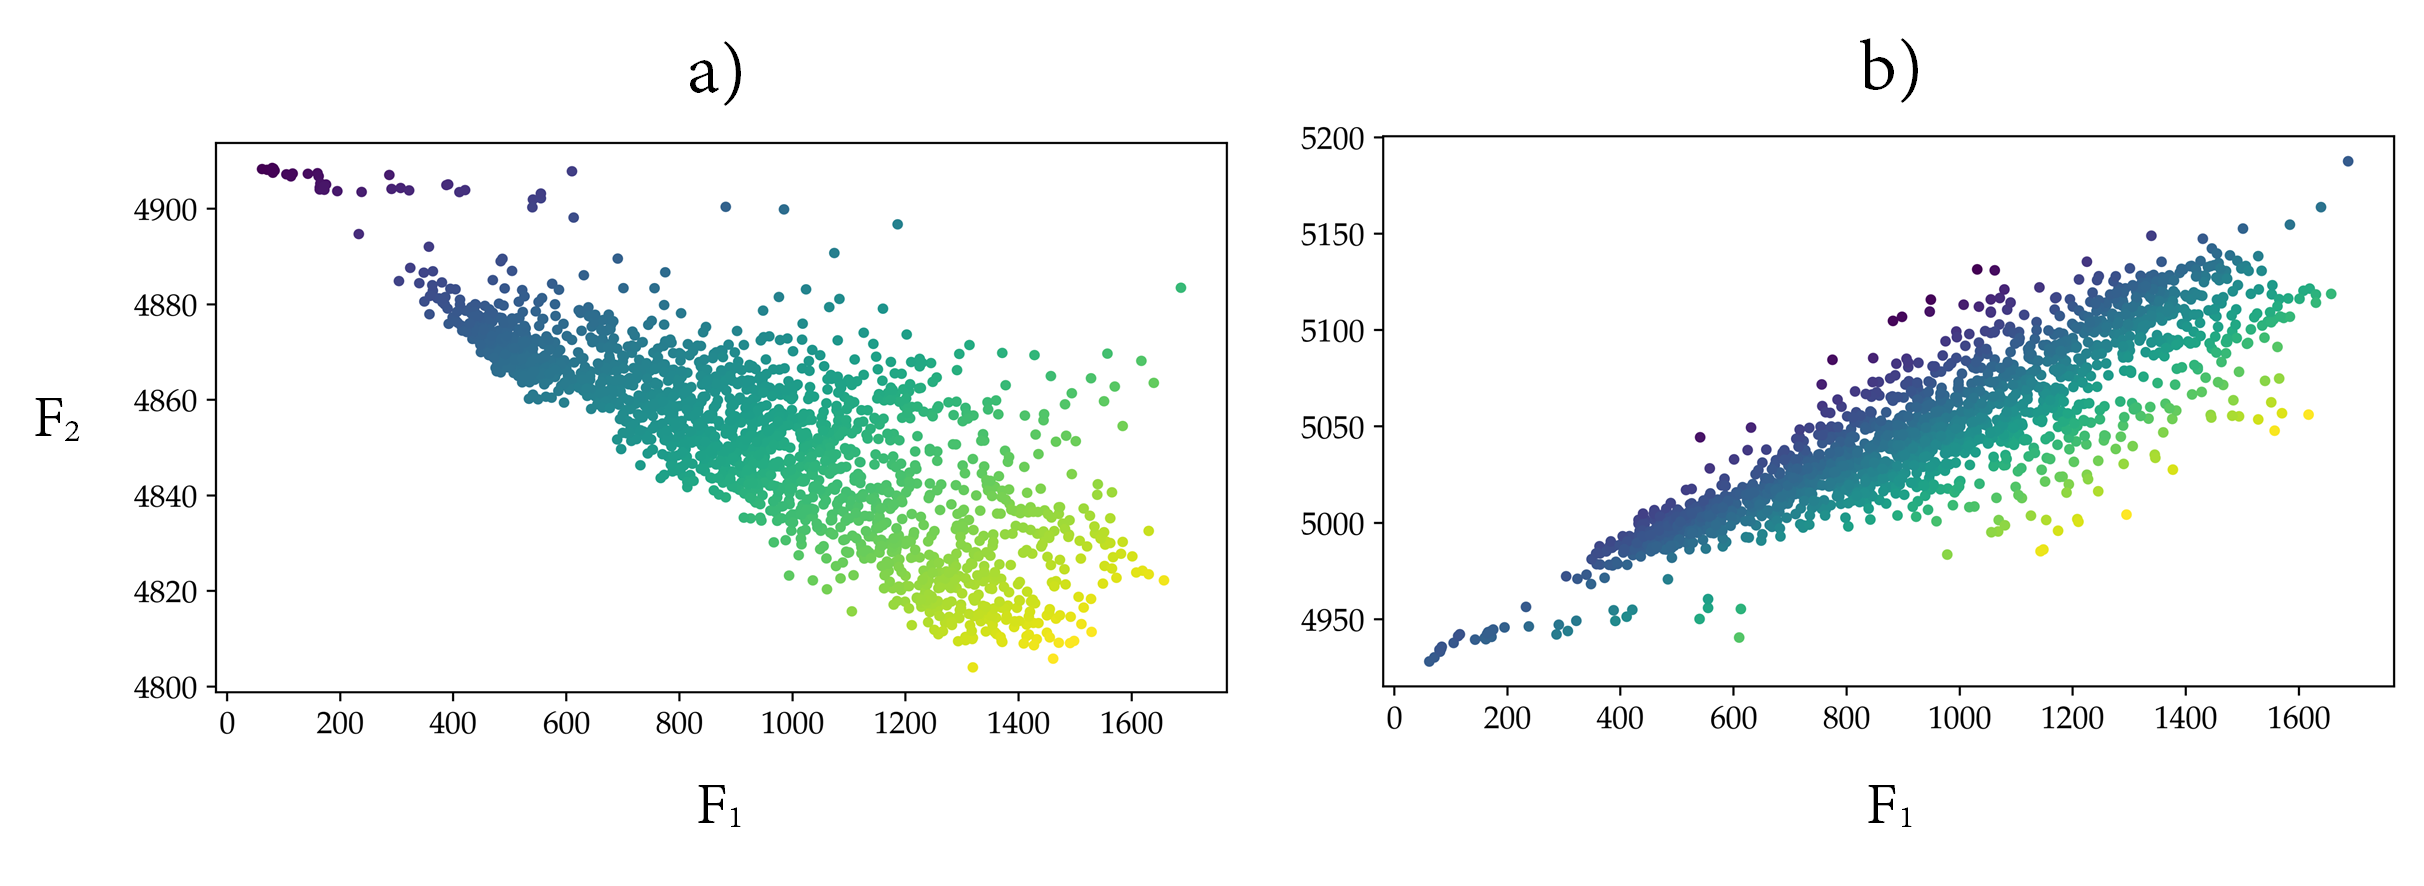
\includegraphics[width=\linewidth]{figs/lidar_optimization/f2_sampling.png}
	\caption{$F_1$ and $F_2$ results from uniformly sampling a 3D environment. The first image depicts how $F_2$ behave with the proposed formula ($F_2$ must be minimized, whereas $F_1$ is intended to be maximized). The second plot does not remove the optimal average distance of collided polygons.}
	\label{fig:f2_sampling}
\end{figure}

\subsection{Level of overlap}

The $F_2$ metric is better suited for achieving local improvements, whereas $F_1$ fits better on the selection of the minimum number of locations providing better scene coverage. However, none of these metrics considers the overlapping of individual scans, despite it being required to guarantee they can be combined in post-processing. To this end, features visible in one scan should also appear in other close scans. With this objective, the $F_3$ metric defined in Equation \ref{eq:overlap_metric} measures the overlapping area between two \acrshort{lidar} scans, indexed as $i$ and $j$, and depicted as circumferences with a fixed radius, $r$.  
\begin{align*}
    A_{i, j} =& \left(r_{i}^{2} \cos^{-1}(\frac{d_i}{r_{i}}) - d_i \sqrt{r_{i}^2 - d_{i}^{2}} +\right. \\
    &\left.+ r_{j}^{2} \cos^{-1}(\frac{d_j}{r_{j}}) - d_j \sqrt{r_{j}^2 - d_{j}^{2}}\right)\\  
    A_{i, j, r_i = r_j} =& 2\left(r^{2} \cos^{-1}(\frac{d}{2r}) - \frac{d}{2} \sqrt{r^2 - \left(\frac{d}{2}\right)^{2}}\right)\\
    \textit{F}_{3_{i, j}^\theta} =& \frac{A_{i, j}}{\pi r_{i}^2} \hspace{1mm} | \hspace{2mm} i, j = 1, 2, ..., \abs{P_c}
    \numberthis \label{eq:overlap_metric}
\end{align*}
where $d$ is the distance from two locations ($d = d_i + d_j$) and $r$ is the \acrshort{lidar} maximum range, which was previously clamped to account for the accuracy loss from distance. Note that $r$ is the same for every scan ($d_i = d_j$).

\begin{marginfigure}[.0cm]
    \centering
    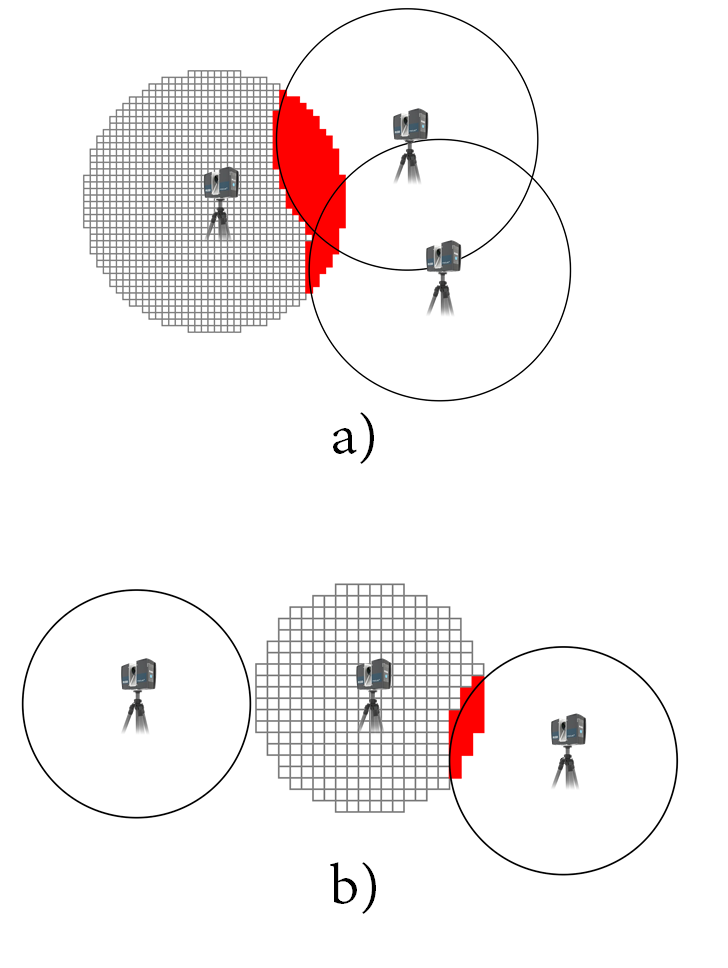
\includegraphics[width=\linewidth]{figs/lidar_optimization/loo.png}
	\caption{Grid occupancy in two different configurations. a) Grid with higher resolution and three overlapping circumferences, and b) sparser grid with only two overlapping circumferences.}
	\label{fig:loo_example}
\end{marginfigure}
The main drawback of Equation \ref{eq:overlap_metric} is that it does not account for the overlapping of previously added locations. To handle this, the occupancy of each \acrshort{lidar} scan is represented using a 2D grid that is filled with points sampled from other scans. Hence, the estimated overlap is given by the number of voxels occupied divided by the overall number. If $d \geq d_1 + d_2$, the sampling can be omitted since both locations do not overlap. Yet, Equation \ref{eq:overlap_metric} helps to establish a ranking of candidate solutions, thus measuring how helpful is every scan to achieve the required overlapping. However, ranking locations by their degree of overlap leads to selecting those with the highest overlap instead of the required one. Accordingly, Equation \ref{eq:loo} ranks locations by their distance to the required overlap. With this approach, solutions that offer a higher overlap than the required one are preferred over those below. To guarantee this, the most significant bit of preferred locations is set to one. Due to the sampling strategy, the accuracy of the overlapping estimations depends on the grid subdivision as well as on the number of sampled points belonging to another \acrshort{tls} scan, as depicted in Figure \ref{fig:loo_example}.
\begin{gather}
    \label{eq:loo}
    \begin{aligned}
        \textit{F}_{3_{i, j}} &=
        \begin{cases}
            \left(r - \left|\psi - \textit{F}_{3_{i, j}^\theta}\right|\right) \BitOr{1 \ShiftLeft 32} &\textit{F}_{3_{i, j}^\theta} \geq \psi\\
            r - \abs{\psi - \textit{F}_{3_{i, j}^\theta}} &\text{otherwise}
        \end{cases}
    \end{aligned}
\end{gather}
with $\psi \in [0, 1]$ being the required overlapping.

Following this approach, the required overlapping is guaranteed for every solution. Still, another shortcoming is the existence of disjoint sets as a result of selecting the best $n$ solutions with a greedy algorithm. Similarly, these flaws can be detected using a disjoint set. New solutions, which belong at least to a disjoint set, are selected according to their distance to another disjoint set and the value of $F_3$, as proposed in Equation \ref{eq:disjoint_set_metric}. The stop criteria are conditioned by the number of disjoint sets, which should be one, and the number of scans, which limits the number of available solutions. The procedure to combine disjoint sets is the following:
\begin{itemize}
    \item First, the closest disjoint sets are selected, as well as the two closest solutions within both of them, $p_o$ and $p_d$.
    \item Then, solutions overlapped with the first location are sorted according to the expression in Equation \ref{eq:disjoint_set_metric}, which must be maximized. 
    \item The new \acrshort{lidar} location is linked to the first solution, which is known to be overlapped, whereas the second solution is only linked whether the overlapping is higher than zero. 
    \item New solutions are also checked to ensure the required overlapping.
\end{itemize}
\begin{align*}
    g(p_o, p_d, p_i) = \left(\frac{d(p_o, p_d) - d(p_i, p_d)}{d(p_o, p_d)} \textit{F}_{3_{o, i}}\right)
    \numberthis \label{eq:disjoint_set_metric}
\end{align*}

\subsection{Point sampling}

During pre-processing, polygons are iteratively sampled to generate uniformly distributed point clouds. Then, the average distance of every point in comparison with the rest is calculated. The overall average distance for a polygon is defined in Equation \ref{eq:mean_distance}. The Euclidean distance is used by default, although it can be exchanged by any other distance function. Note that $\abs{P}-1$ is used instead of $\abs{P}$ to not take into account the distance of points with themselves in an efficient way. 
\begin{align*}
    d_{\mu} = \frac{\sum_{i=1}^{\abs{P_t}} \frac{\sum_{j=1}^{\abs{P_t}} d^{2}(p_{i} - p_{j})}{\max\left(\abs{P} - 1, 1\right)}}{\max\left(\abs{P}, 1\right)}
    \numberthis \label{eq:mean_distance}
\end{align*}
where $P_t$ represents a set of points in a triangle $t$ and the inner summation computes the Euclidean distance for 3D points.

\begin{marginfigure}[0cm]
    \centering
    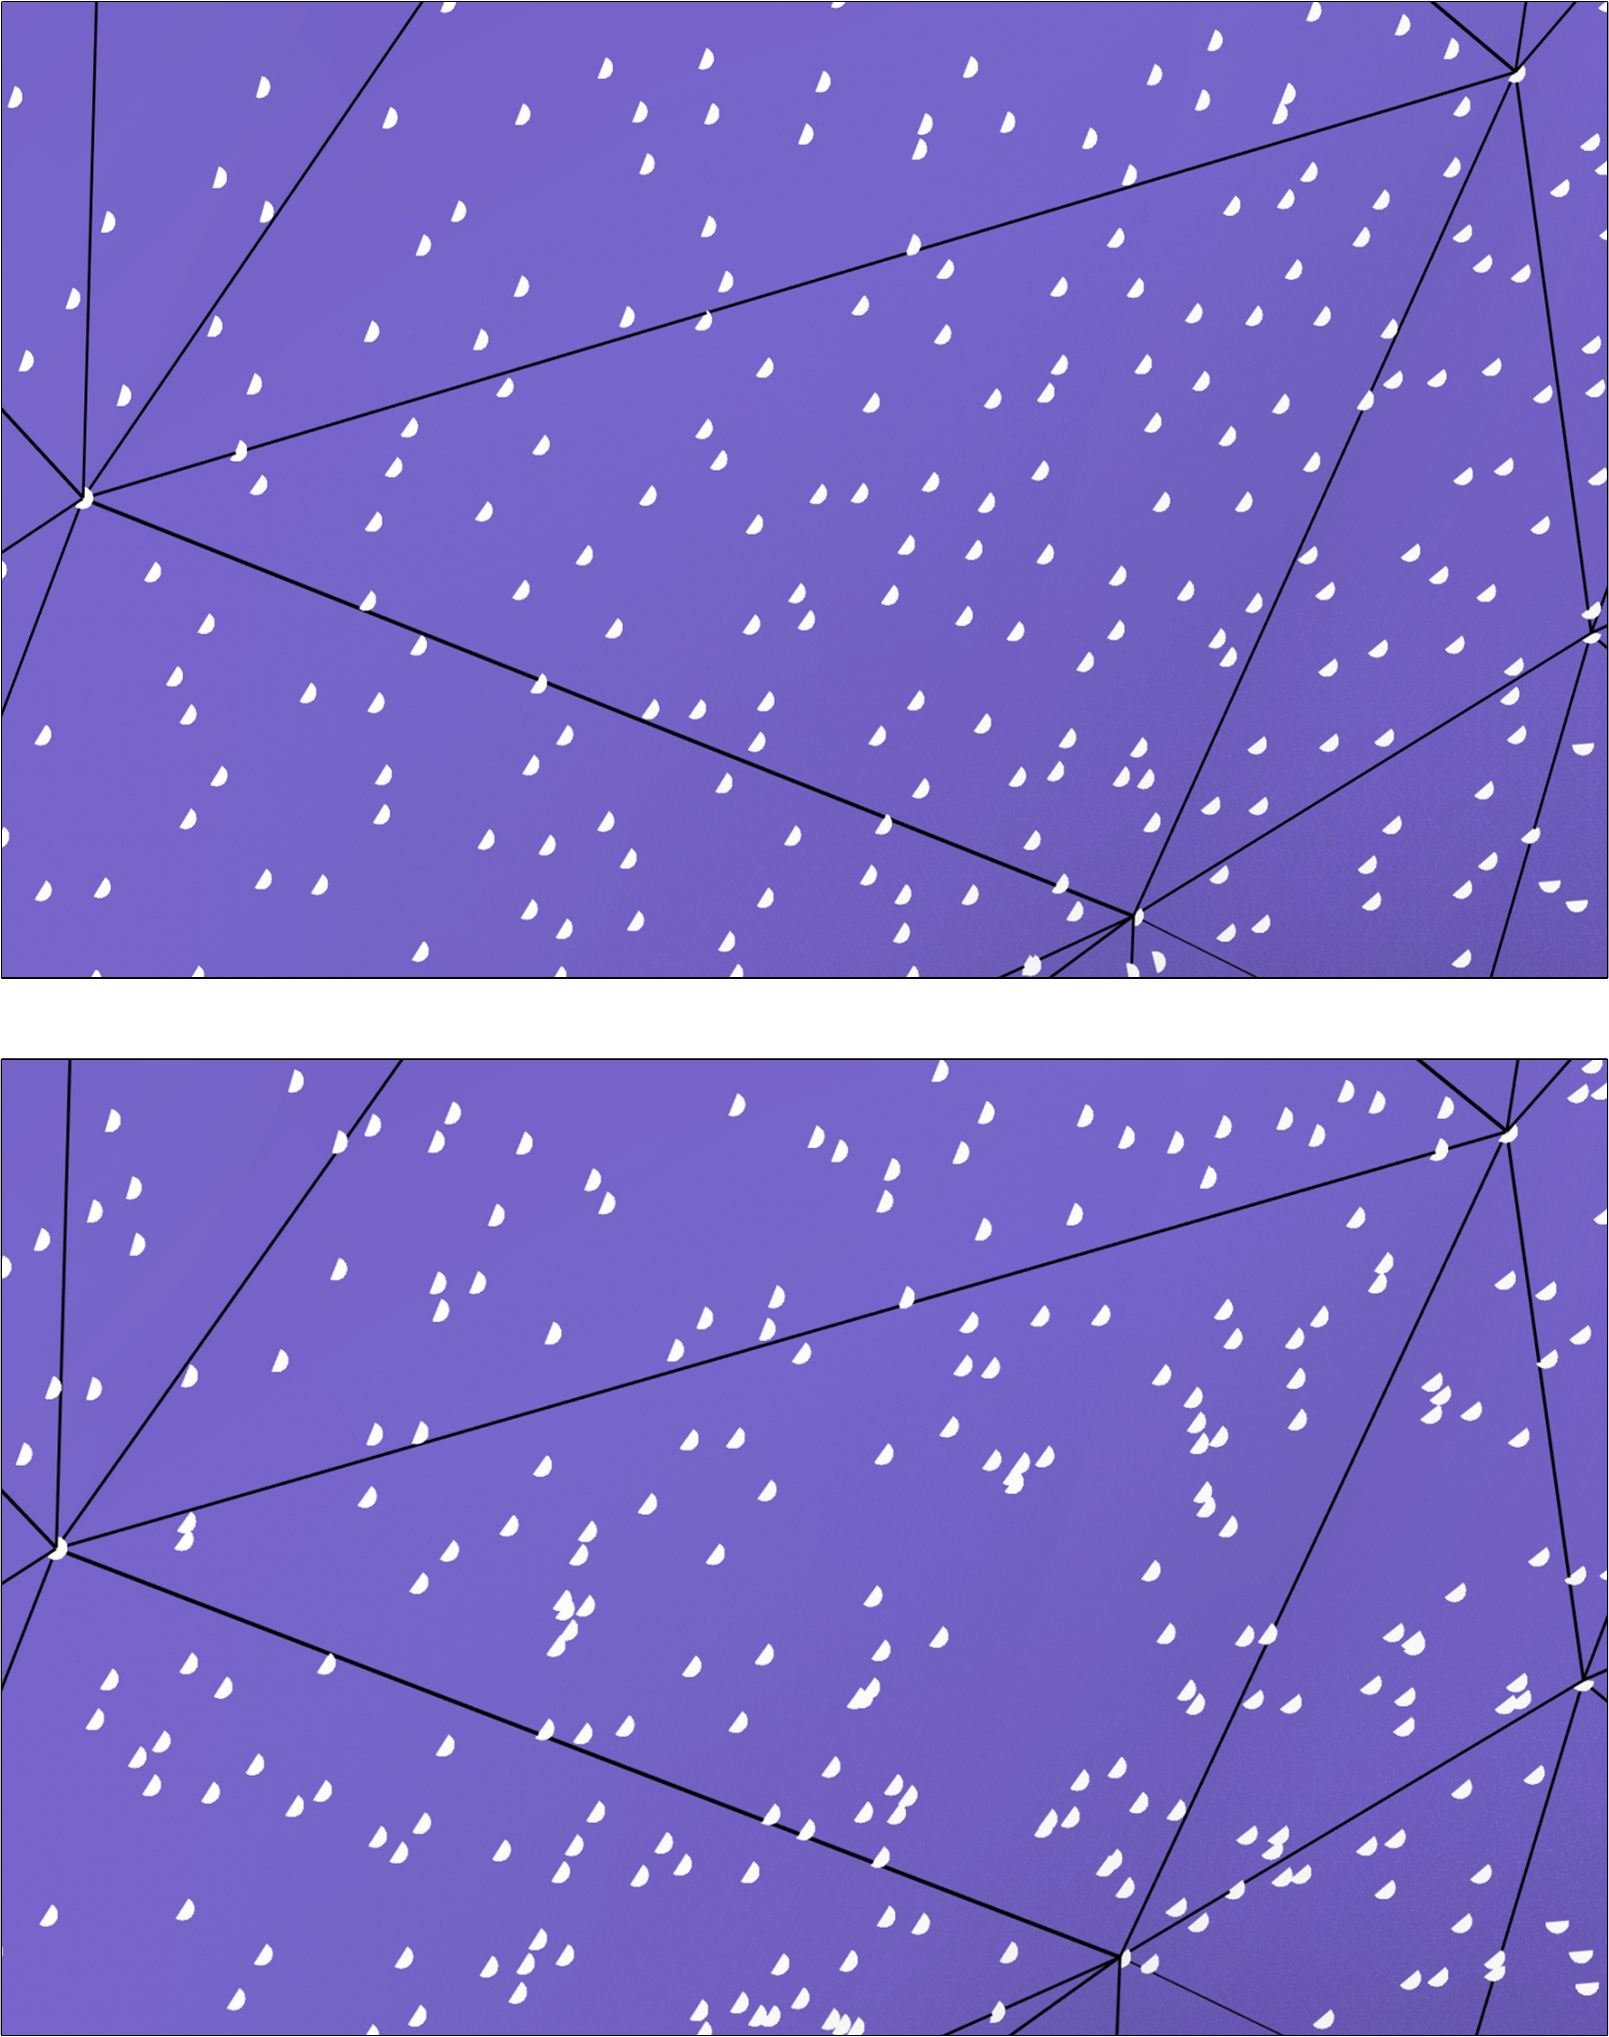
\includegraphics[width=\linewidth]{figs/lidar_optimization/point_sampling.png}
	\caption{Comparison of polygons sampled using the Halton sequence and the C++ built-in random uniform distribution.}
	\label{fig:point_sampling}
\end{marginfigure}
Although built-in random uniform distributions are available in most language libraries, these are mainly based on pseudo-random sequences such as those used for Classic Monte Carlo integration (\acrshort{cmc}). They provide good quality estimations, but they require a large number of samples and have a higher response time \cite{marques_optimal_2019}. The latter drawback is irrelevant in this case study since only a few points will be sampled from each triangle, with the number being conditioned by the polygon area. However, these distributions generate point clouds far from the expected uniformity. Instead, the \acrshort{qmc} method is based on well-distributed deterministic sampling patterns that provide better results for our objective. More specifically, the Halton sequence was used to calculate the quasi-optimal mean distance within polygons \cite{burkardt_halton_2010}. Figure \ref{fig:point_sampling} shows the outcome of sampling points with the C++ built-in random uniform distribution and the proposed \acrshort{qmc} sequence.

Either from pseudo-random or \acrshort{qmc} sequences, two parametric values ($u$, $v$) are generated to sample a triangle surface. Equation \ref{eq:triangle_parametric} shows the formula for generating a point within a triangle defined through its three vertices ($p_1$, $p_2$, $p_3$) with $u, v \in [0, 1]$. 
\begin{align*}
    p_{s} = (1 - \sqrt{u}) p_1 + (\sqrt{u} (1 - v)) p_2 + (v \sqrt{u}) p_3
    \numberthis \label{eq:triangle_parametric}
\end{align*}

Note that a significant drawback of this approach is that sparse scans with all their points gathered in a small area are also evaluated as appropriately uniform. To solve this, the triangle vertices were included as part of the point set, $\abs{P}$, thus penalizing scans biased towards certain parts of polygons.

\subsection{Solution initialization}

The initial search space must be partitioned to obtain the first solutions ($N$) over polygons that are interactively marked as ground. From the collected ground planes, the 2D \acrshort{aabb} is estimated to restrict the search space. However, an \acrshort{aabb} does not adjust well to most of the possible shapes, and may still lead to instancing solutions out of the floor model. Therefore, candidate locations must be evaluated to ensure that:
\begin{itemize}
  \item \textbf{The location is over a ground polygon}. To verify this, a ray is cast towards -\textit{Y} in the \acrshort{bvh}. Ground polygons are transferred to the \acrshort{gpu} and their Id is compared against the nearest collision.
  \item \textbf{The sensor is not located over non-ground planes}, e.g., furniture placed between the floor and the \acrshort{lidar} sensor. \textit{m} points are sampled around the candidate location, using a radius $r$ and casting $m$ rays with $-\vec{Y}$ direction. The location is discarded whether any of the $m$ rays have their nearest collision in non-ground-labelled items. Both $r$ and $m$ can be configured.
  \item \textbf{The sensor is not located close to building walls and furniture}. It cannot be placed over items, nor next to them, thus guaranteeing a safety distance. Hence, four additional rays are cast using \{\textit{X, -X, Z, -Z}\} vectors.
\end{itemize}

At least two ways to initialize solutions were integrated: random and uniform sampling. The uniform sampling utilizes a 3D matrix bounded by the ground \acrshort{aabb}, whereas the sensor height is limited by the \acrshort{lidar}'s maximum and minimum height. The \acrshort{lod} of the partitioning is parameterized with the voxel size; a lower size provides a better \acrshort{lod} and a higher number of solutions. Otherwise, solutions can be randomly distributed to provide a less exhaustive initialization. The latter approach explores fewer solutions, scattered throughout the scene using a random uniform distribution. Note that in this approach uniformity is not a must; instead, it is avoided to provide an alternative to the uniform, grid-like, sampling. Then, the set $N$ is either enhanced (spatial search), subsampled (greedy algorithm) or narrowed with bit sets (\acrshort{ga}). 

\section{Spatial search}

This section explains how the initial solutions, $N$, change and improve to provide a wider space exploration, instead of simply relying on the starting locations. However, metrics aimed at improving scans do not have any knowledge concerning overlapping. The following searches work according to the $F_2$ metric from Equation \ref{eq:uniformity_error}.

\subsection{Solution neighbourhood}

\begin{marginfigure}[-8.cm]
    \centering
    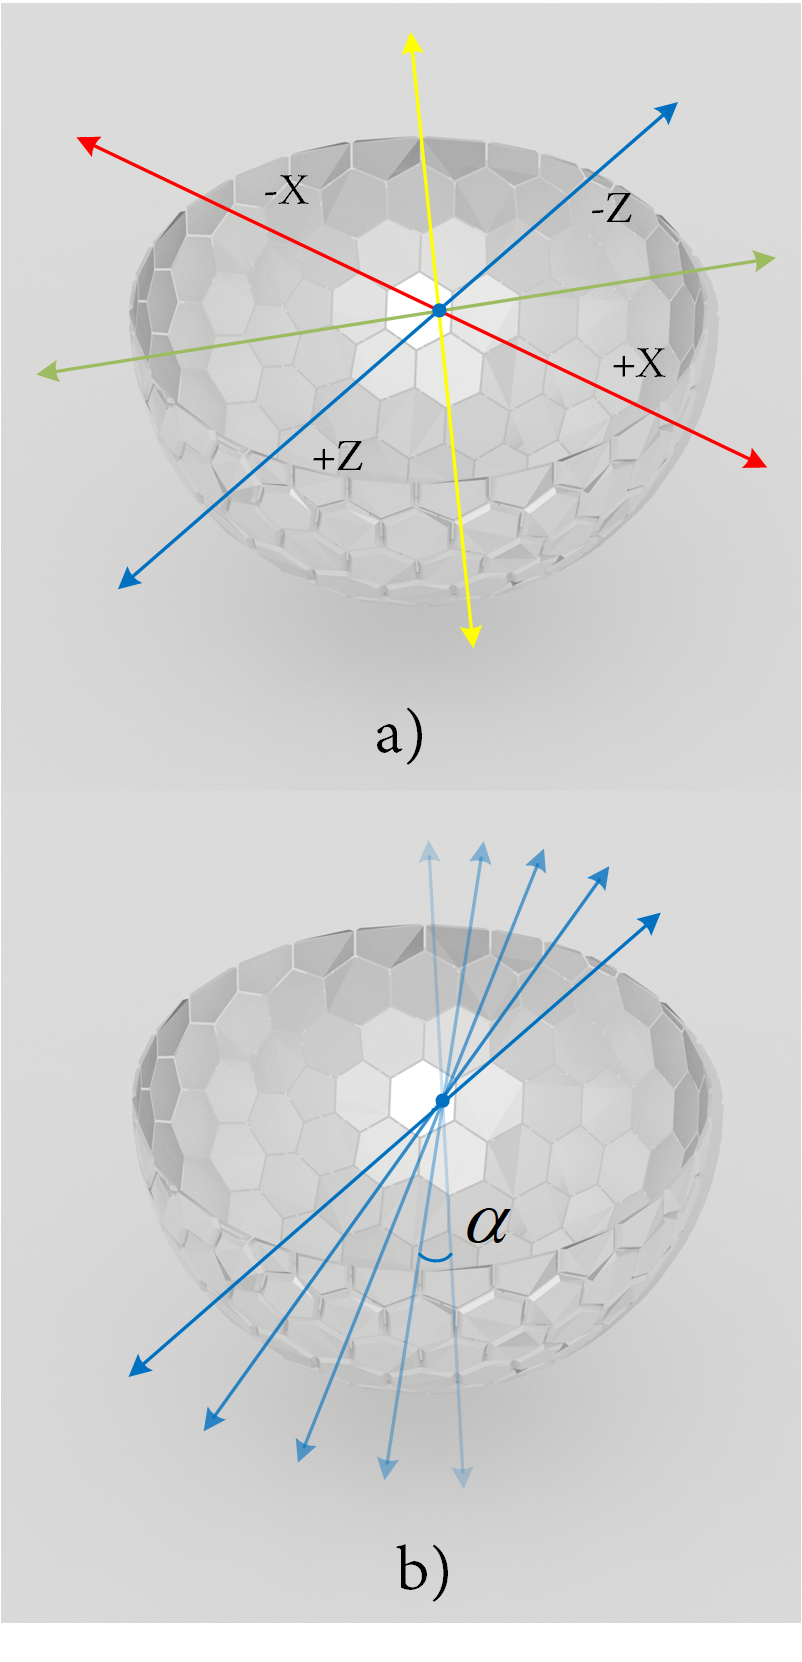
\includegraphics[width=\linewidth]{figs/lidar_optimization/neighbour_search.png}
	\caption{Overview of gradients for a 2D neighbour search. a) A fixed approach generates eight vectors, whereas b) the subsampling of a circumference can be performed with a variable resolution.}
	\label{fig:neighbour_search}
\end{marginfigure}
Neighbourhood exploration is aimed at locally enhancing candidate scans. The neighbourhood of a scan is a set of 3D points close to the sensor location. Discretization poses several challenges since there is an infinite number of possible translations. The first approach is to downscale the neighbourhood to 14 unitary vectors (six faces and eight corners of a cube). Otherwise, it can be discretized by uniformly subsampling a unit sphere, thus obtaining a buffer of gradients whose length depends on the user-defined sampling resolution. Furthermore, unit vectors can be down- and up-scaled with a step length: larger changes may omit good candidates, and the contrary may be too exhaustive. Figure \ref{fig:neighbour_search} illustrates the gradient vectors that help to explore the contiguous space in 2D: the first scenario has fixed partitions, whereas the second depends on the user-defined resolution.

\subsection{Greedy algorithm}

The traditional local search (\acrshort{ls}) is here referred to as a Greedy algorithm and helps to rapidly survey the neighbourhood. The surrounding points are evaluated and sorted according to the results of the metrics. Solutions are iteratively improved by adopting the location of the best neighbour if any improves the current location. Otherwise, this approach gets stuck on local minima and terminates. The termination criteria also contemplate reaching a maximum number of iterations. Re-visiting previously explored locations is avoided with the dot product ($\cdot$) between the gradient being evaluated and the previous one ($f(\hat{g}_1, \hat{g}_2) = \hat{g}_1 \cdot \hat{g}_2$). Hence, a gradient is considered to be already explored whether $f(\hat{g}_1, \hat{g}_2) < \epsilon - 1$, with $\epsilon$ being a small value such as $2^{-16}$ that avoids errors derived from comparing floating-point data. Note that this test is very efficient and copes with immediate loops; however, loops with a deep higher than one are possible.

\subsection{Simulated annealing}

\acrshort{sa}, in contrast to the greedy approach, avoids getting stuck in local optima. To this end, neighbours with worse fitness than the current solution are accepted under probabilistic criteria. The acceptance ratio is modelled as a temperature value, $T$, which is first initialized and downscaled iteratively according to a cooling factor \cite{wieckowski_finding_2020}. In this work, it is configured using the traditional exponential formula defined in Equation \ref{eq:simulated_annealing_exp}: 
\begin{gather}
    \label{eq:simulated_annealing_exp}
    \begin{aligned}
        p(f') =
        \begin{cases}
            \exp(\frac{f'-f}{T}) &f'-f \geq 0\\
            1 &f'-f < 0
        \end{cases}
    \end{aligned}
\end{gather}
given that $f'$ and $f$ are two fitness values from a new solution and the current one, respectively, in a minimization problem. Consequently, a random uniform distribution is also applied to determine whether a worse solution is accepted. The stop criterion depends on a threshold temperature and a maximum number of iterations.

\subsection{Tabu search}

A trivial improvement of \acrshort{ls} is given by a tabu search (\acrshort{ts}), where the already processed locations are avoided with the so-called tabu moves. The explored solutions cannot be re-explored and therefore, all the neighbours may be tabu. In this case, the solution space can be re-initialized. The very same scenario is achieved if every neighbour worsens the fitness of the current location, or a maximum number of iterations is reached without any improvement. The main shortcoming of 3D explorations is how to store tabu moves, which was approached using a 3D regular grid of variable resolution. Hence, a neighbour is considered tabu when the target point falls in a tabu voxel. Given the step size of neighbour explorations, $n_l$, an appropriate voxel size is given by $f \cdot n_l$, with $1 < f < 2$.

\section{Genetic algorithm}

Genetic algorithms operate over previously enhanced solutions to find an optimal subset. This sort of algorithm is inspired by nature on how to handle populations that evolve and improve over time. Accordingly, it combines exploration and exploitation phases \cite{vannucci_genetic_2020}. Regarding our case study, this metaheuristic helps to reduce the setup complexity while still providing dense coverage. In comparison with memetic algorithms, the first stage aims to improve individual locations guided by an exploration of surrounding areas, without evaluating the scene coverage. Yet, the proposed $F_2$ metric weights non-scanned polygons. After this, a \acrshort{ga} finds the optimal solution regarding the scene coverage. To this end, a slight variation of the previously proposed $F_1$ metric is here proposed. The complete procedure is depicted in Figure \ref{fig:genetic_overview}, whose stages are following detailed:

\textbf{Initialization of population}. The solution space is first populated with $p$ chromosomes of size $n$, each one with a random number of activations (\acrshort{lidar} locations). Hence, variety is ensured by avoiding populations with a fixed number of activated bits.

\begin{marginfigure}[-3.0cm]
    \centering
    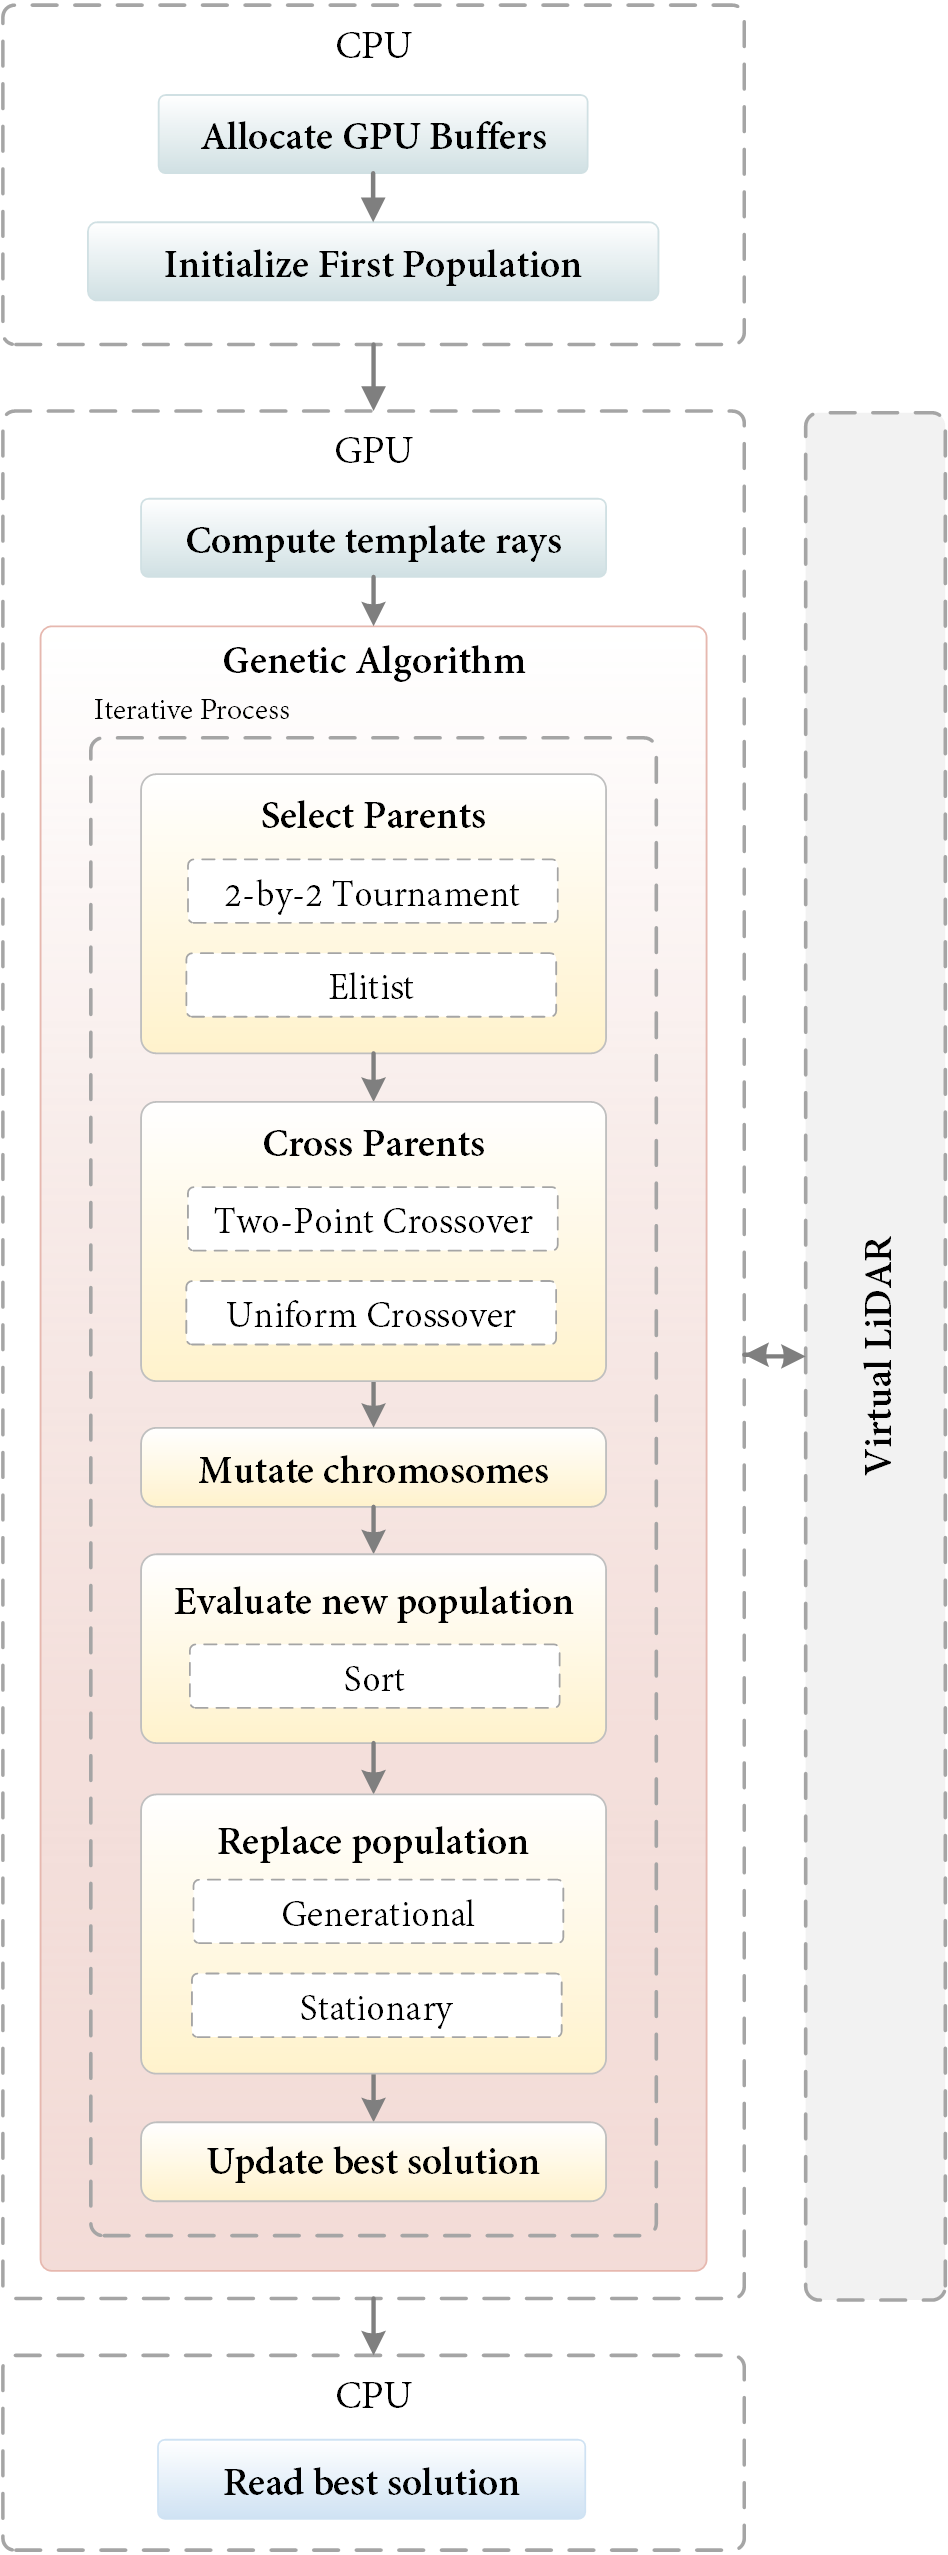
\includegraphics[width=\linewidth]{figs/lidar_optimization/genetic_overview.png}
	\caption{Overview of \acrshort{ga}s on the evaluation of the best combination of spatial \acrshort{lidar} setups.}
	\label{fig:genetic_overview}
\end{marginfigure}
\textbf{Compute template rays}. Template rays are intended to describe how rays traverse the space from a default \acrshort{lidar} location, which is known to be at $0^3$. These rays are generated according to the specifications of a commercial \acrshort{lidar} sensor. Then, the \acrshort{lidar} point clouds are simulated from this set of rays. Template rays are only transferred once to the \acrshort{gpu}, rather than calculating and transferring them for every location to be checked. The \acrshort{gpu}-based \acrshort{lidar} simulation proposed in previous chapters was simplified to provide only the first collision to favour both replicability and performance. 

\textbf{Parent selection}. The aim of this stage is to select the $s$ most promising individuals for the subsequent crossover. Two different selections are here proposed. First, the 2-by-2 tournament allows selecting good solutions, although they may not be in the top-most $s$. This approach favours the variability of later populations. On the contrary, the elitist selection chooses the best individuals from the current population.

\textbf{Crossover}. Previously selected parents are combined to generate the next population. Parents can be mixed by selecting a crossing point which split each chromosome into two parts which are combined to build offspring. Another approach is to randomize the crossover by utilizing random values which determine the parent from which each gen is obtained ($p_{1_{i}}$ if $r_i \leq 0.5$, $p_{2_{i}}$ otherwise). There is only a non-valid solution, given by the zero chromosome ($0^n$), which is easily handled by randomly altering a bit.

\textbf{Mutation}. Mutations include minor variations in new generations. This stage is parameterized by the number of mutable individuals and genes within each one. No restrictions are considered regarding the number of activations, and therefore, mutations simply activate or deactivate some random bits.

\marginnote[.5cm]{
	\begin{equation}
    \textit{F}_{1} = \frac{\sum_{s=1}^{\abs{S}} 1[t_s \in \{L_1, ..., L_k\}]}{\sum_{g=1}^{n} c_g}
    \label{eq:metric_count_alt}
	\end{equation}
}
\textbf{Evaluation of new population}. The fitness of every new solution is estimated based on the computed returns. Accordingly, solutions covering more polygons are more likely to be selected as parents in the following iterations. However, this approach favours activating every bit in every chromosome. Instead, the previously proposed $F_1$ metric is modified according to Equation \ref{eq:metric_count_alt} by also accounting for the number of activated bits within a chromosome ($c_g$). With this new metric, the genetic algorithm is intended to reach the maximum number of polygons with the minimum number of scans.

\textbf{Replace population}. New and previous populations are then mixed following the generational or stationary approach. The generational approach replaces parents with their offspring, whereas the stationary algorithm replaces the worst individuals with the new population whether they improve current solutions.

\textbf{Update best solution}. It is noteworthy that even this minor operation must be performed in the \acrshort{gpu}, as the reading transfer would lead to a huge delay in the \acrshort{ga} response time.

\section{Interactive tools}

This section presents some tools intended to facilitate the configuration of the scenario and the algorithm.

\subsection{Picking of scannable building levels}

The described \acrshort{p4s} method is not restricted to buildings with a single level. Indeed, it has been evaluated in realistic buildings with several of them. However, the planning must be addressed individually. The selection of floor-labelled polygons is interactively performed with ray-casting, thus obtaining the intersected primitive in real time. The result is computed by casting a ray whose direction is given by the user's viewpoint and a 3D position, which is computed by unprojecting the camera matrix to a 2D point within the application canvas. The first collided model is obtained traversing the \acrshort{bvh} and pushed into the ground list. With this regard, Equations \ref{eq:unprojection1} and \ref{eq:unprojection2} show how to unproject a 2D canvas point to 3D.
\begin{align*}
    p_{\textit{3D}} &= \hspace{.5mm} \inv{\left(P \cdot V\right)} \cdot \hspace{1mm} \left[\frac{p_{\mathit{2D}_x}}{c_x}2 - 1,  \frac{p_{\mathit{2D}_y}}{c_y}2 - 1, 0, 1\right]^T
    \numberthis \label{eq:unprojection1}\\
    p_{\textit{3D}} &= \frac{p_{\textit{3D}}}{p_{\textit{3D}_w}}
    \numberthis \label{eq:unprojection2}
\end{align*}
where $(p_{\textit{2D}_x}, p_{\textit{2D}_y)}$ is the canvas point, $P$, $V$ are the camera projection and view matrices, respectively, $(c_x, c_y)$ is the canvas size, and $p_{\textit{3D}}$ is a 4-tuple describing the projection coordinates.

\subsection{Pipeline design}

Spatial searches and \acrshort{ga}s can be concatenated to iteratively improve the starting solutions. Hence, this pipeline is not solely limited to applying \acrshort{ls} + \acrshort{ga}s. Instead, a flexible pipeline was implemented to omit stages if necessary and even concatenate several \acrshort{ls}. The pipeline design was facilitated using a node editor as the one depicted in Figure \ref{fig:optimization_node_editor}. Greedy, \acrshort{sa}, \acrshort{ts} and \acrshort{ga} nodes can be chained one after another, and even the spatial searches were parameterized to support the narrowing of solutions according to their fitness and the required number. Note that, by default, the maximum number of solutions is not required; instead, it is intended to be implicitly computed in the \acrshort{ga}.

\begin{figure*}[ht]
    \centering
    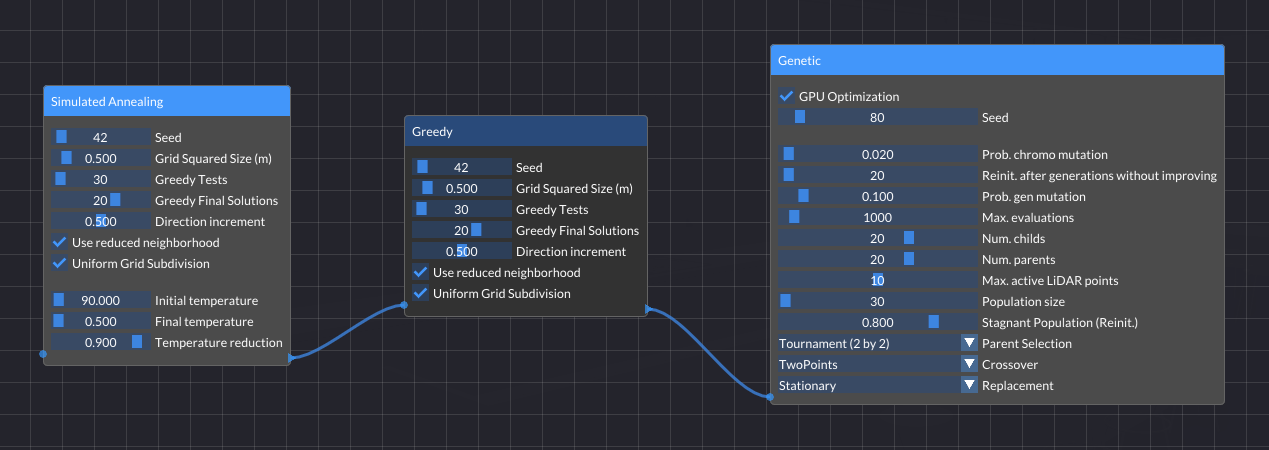
\includegraphics[width=\linewidth]{figs/lidar_optimization/optimization_node_editor.png}
	\caption{Showcase of a node editor chaining \acrshort{sa}, Greedy and \acrshort{ga} nodes. }
	\label{fig:optimization_node_editor}
\end{figure*}

\section{Results and discussion}

\begin{figure*}
    \centering
    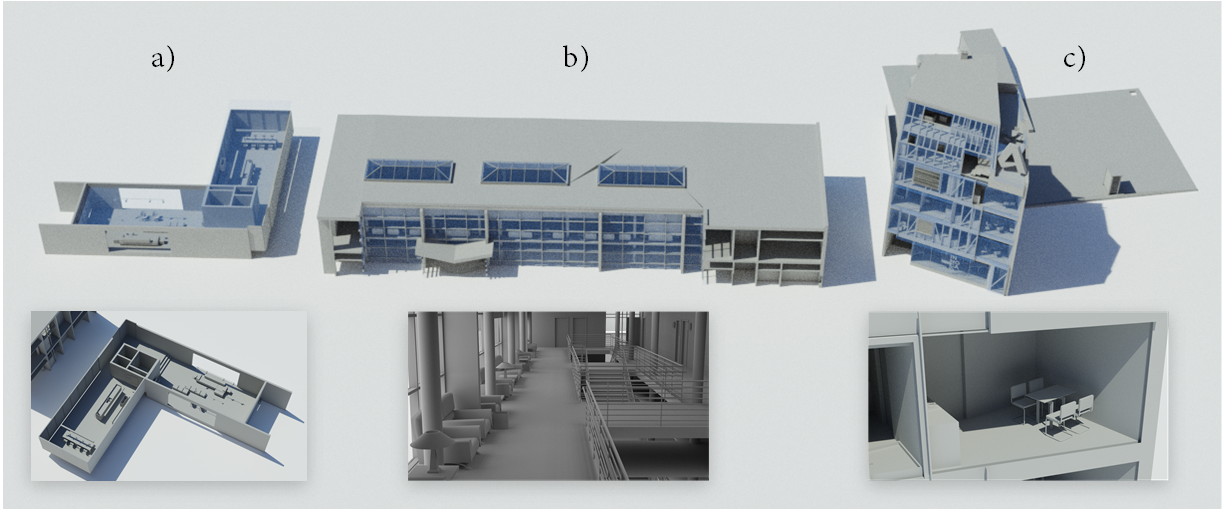
\includegraphics[width=.95\linewidth]{figs/lidar_optimization/evaluation_scenes.png}
	\caption{Three different environments authored by Autodesk Revit \textregistered \hspace{.5mm}. a) A basement with 130k triangles ($20 \times 4 \times 21$\si{\meter}), b) a school with 500K triangles ($44 \times 24 \times 32$\si{\meter}) and c), an office building with 2.7M triangles ($16 \times 8 \times 49$\si{\meter}). }
	\label{fig:bim_environments}
\end{figure*}

The proposed optimization has been tested against three different scenes from commercial software (see Figure \ref{fig:bim_environments}), with a size ranging from 130k to 2.7M polygons. Although there exist a few studies concerning \acrshort{p4s} in 3D, their implementations are not available. Consequently, the carried out experiments are focused on evaluating the results of metrics and the performance speedup in comparison with a multi-core \acrshort{cpu}-based approach. The latter version is implemented using \acrshort{openmp} when possible; however, the \acrshort{lidar} simulations are very time-consuming and they were solved in the \acrshort{gpu} in both approaches. The configuration of local searches (\acrshort{ls} from now on) is shown in Table \ref{table:local_search_settings}, whereas \acrshort{lidar} specifications are detailed in Table \ref{table:optimization_lidar_parameters}. All measurements were performed on a PC with AMD Ryzen Threadripper 3970X 3.6 GHz, 256 GB RAM, two NVIDIA RTX A6000 \acrshort{gpu} and Windows 10 \acrshort{os}. 

\renewcommand{\arraystretch}{1.15}
\begin{table}[hb]
\caption{Configuration of parameters concerning greedy, \acrshort{sa} and \acrshort{ts} algorithms.}
\label{table:local_search_settings}
\begin{tabular}{@{}ll@{}}
\toprule
\textbf{Attributes} & \textbf{Value}\\
\midrule
Starting solutions & Grid sampling\\
Number of final solutions & Without restrictions\\
Voxel size & 0.5 \si{\meter} $\times\hspace{1mm}$0.4 \si{\meter}\\
\midrule
Max. number of iterations & 60\\
Max. number of iterations without improvements & 10\\
\midrule
Neighbourhood & Discrete (16)\\
Length of neighbourhood steps ($\Delta$) & 0.05 $\si{\meter}$\\
\midrule
Initial temperature ($T_0$) & 450$^{\circ}$C\\
Temperature decrease ($T_z$) & 0.8 $T_{z-1}$\\
\bottomrule
\end{tabular}
\end{table}
\renewcommand{\arraystretch}{1}

\renewcommand{\arraystretch}{1.15}
\begin{table}
\caption{Specifications of \acrshort{lidar} sensor during optimization, following the commercial device HDL-64E. }
\label{table:optimization_lidar_parameters}
\begin{tabular}{p{0.51\linewidth}p{0.4\linewidth}}
\toprule
\textbf{Attributes} & \textbf{Value}\\
\midrule
Resolution & 4500 $\times$ 64 beams\\
Maximum number of returns & 1\footnote[1]{It has been adapted to reduce the optimization latency.}\\
Maximum range & 5 \si{\meter}\footnote[2]{It has been adapted to improve the accuracy of the results.}\\
Coverage & 360\textdegree x 26.9\textdegree$\hspace{1mm}$(-24.9\textdegree-2\textdegree)\\
Height coverage & [0.5, 2] \hspace{.3mm}\si{\meter}\\
Minimum \textit{xz} distance to items & 0.4 \si{\meter}\\
Vertical tests & r $\gets$ 0.2 \si{\meter}, n $\gets$ 16 rays\\
%Interleaved solution distance & 4 \si{\meter}\\
\bottomrule
\end{tabular}
\end{table}
\renewcommand{\arraystretch}{1}

This section is organized as follows. First, the performance of different \acrshort{ls} algorithms was evaluated regarding $F_1$ and $F_2$ metrics. Then, \acrshort{ls} and \acrshort{ga} algorithms were combined to find the best pipeline, also in terms of metrics. \acrshort{cpu} and \acrshort{gpu} approaches were assessed according to the measured response time, and finally, an experiment was carried out to show the benefits of considering \acrshort{lidar} sensors with variable height.

\subsection{Performance of local searches}

This section shows how local searches improved the $F_2$ results using greedy, \acrshort{ls}, \acrshort{sa} and \acrshort{ts} over the basement scene. The evaluation of the $F_2$ metric for each initial solution is depicted regardless of the best solution observed until such iteration. Although \acrshort{ls} achieved huge improvements, the importance of \acrshort{ga} selection is evidenced by Figure \ref{fig:greedy_results}. It shows the narrowing phase of a greedy algorithm that selects the best $k \gets 30$ scans (red) in a scenario with areas that have disparate geometrical complexity, guided by the minimization of the $F_2$ metric. Hence, most of the selected locations were surrounded by dense geometry, and yet, it managed to cover most of the scene. Similarly, small enclosed rooms, as the zoom-in of Figure \ref{fig:greedy_results}, are not scanned due to their smaller number of polygons.

\begin{figure}
    \centering
    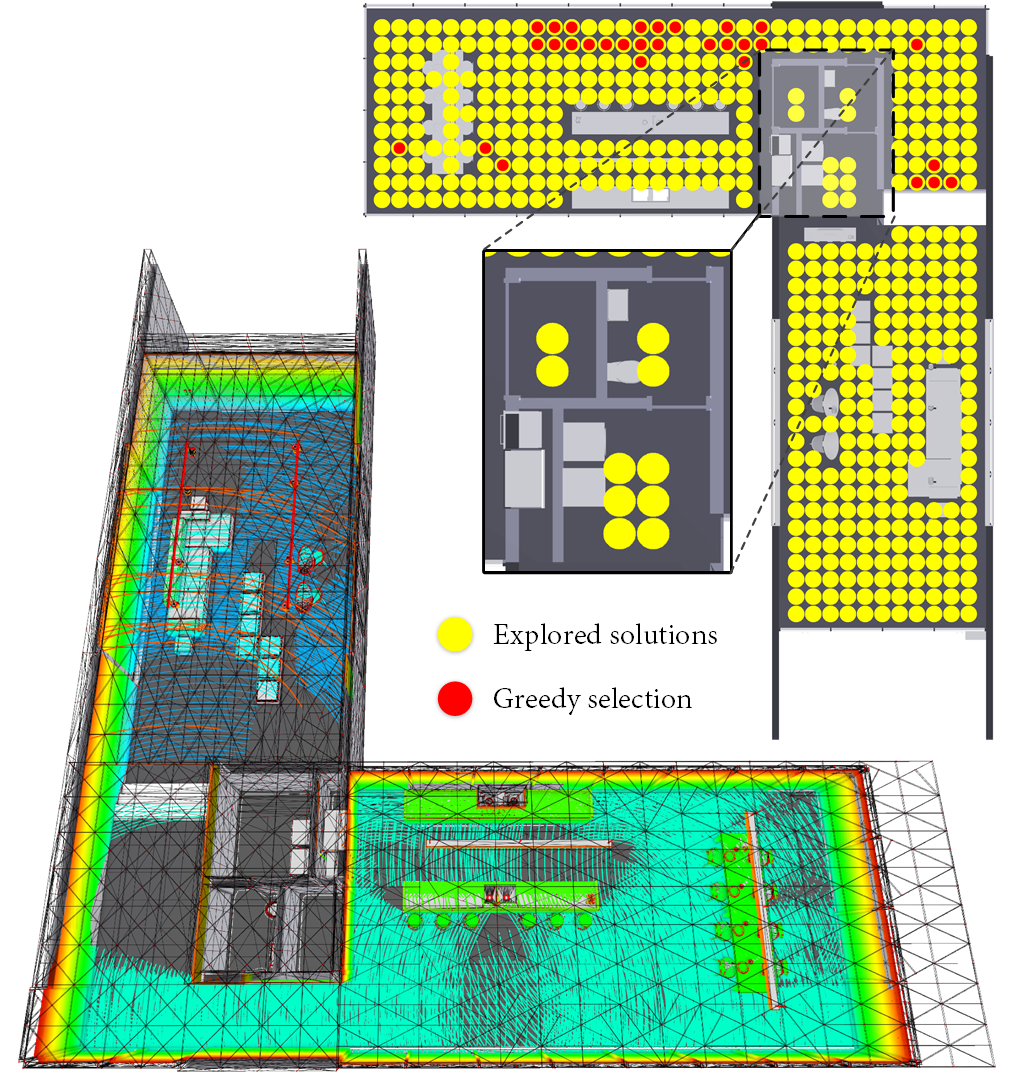
\includegraphics[width=.8\linewidth]{figs/lidar_optimization/greedy_results.png}
	\caption{Selection of the best thirty \acrshort{lidar} scans with a greedy approach in the basement scene.}
	\label{fig:greedy_results}
\end{figure}

\begin{figure*}
    \centering
    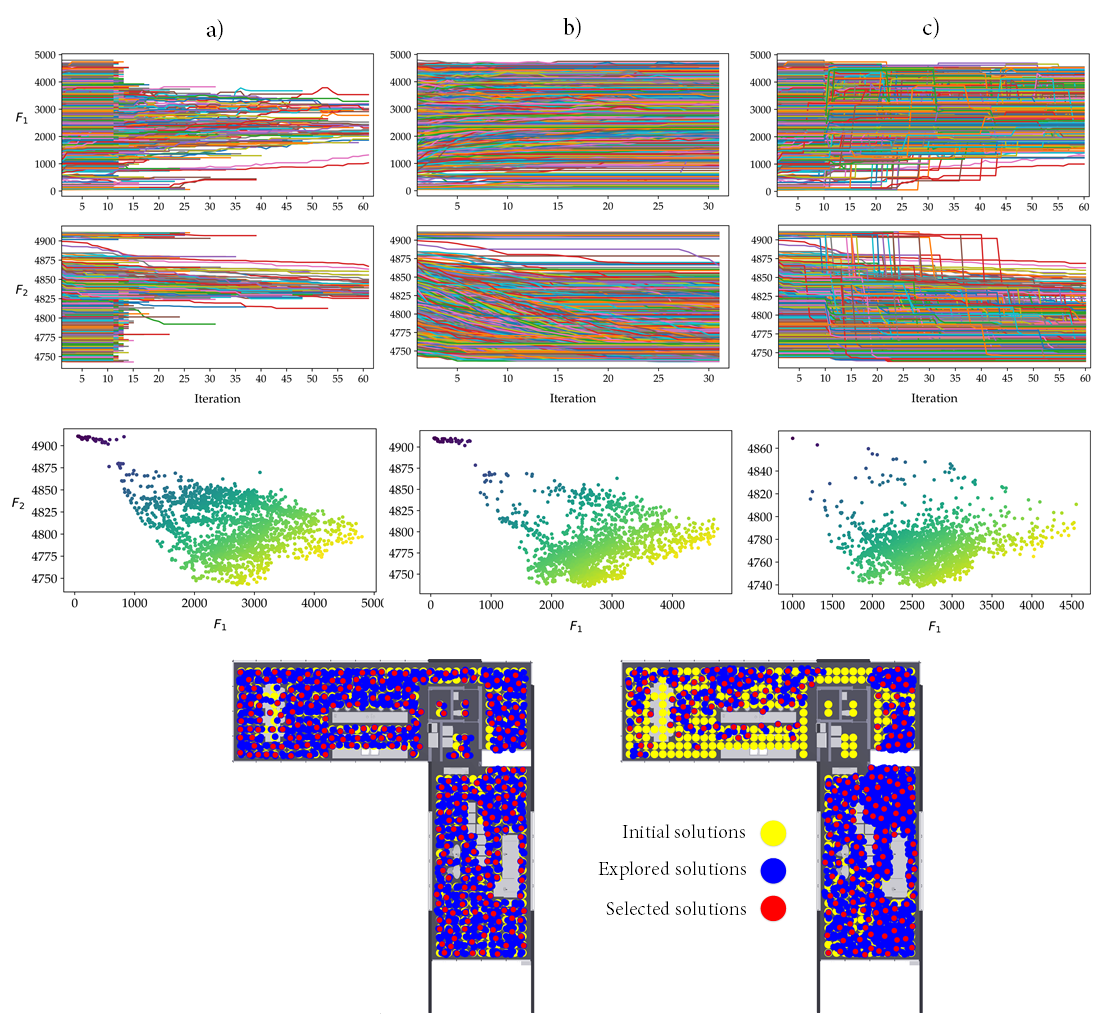
\includegraphics[width=.9\linewidth]{figs/lidar_optimization/local_search_results.png}
	\caption{Optimization obtained using a) naive \acrshort{ls}, b) \acrshort{sa} and c) \acrshort{ts}, showing both $F_1$ and $F_2$ results in a timeline as well as the final distribution. The bottom images show the locations optimized with \acrshort{sa} and \acrshort{ts}, organized into a regular grid and filtered by selecting only one solution per subdivision.}
	\label{fig:local_search_results}
\end{figure*}

From this baseline, Figure \ref{fig:local_search_results} depicts the improvements of initial solutions with different \acrshort{ls}. For that purpose, the $F_1$ and $F_2$ results achieved by individual solutions are depicted during a fixed number of iterations. However, some explorations, such as \acrshort{sa}, finished earlier since the temperature also converged sooner or no better solutions were found. Optimized locations are not narrowed using \acrshort{ga}, and therefore, those depicted are filtered according to a regular grid that allows selecting a single solution per partition.

\textbf{Local search}. As expected from the description of \acrshort{ls}, the explorations of initial solutions finished early, especially for locations that start with low $F_2$ values. Worse solutions than the current one were not accepted, thus rapidly achieving the maximum number of iterations. Also, changes were controlled with a small factor; otherwise, the grid-like sampling turn into a random sampling. Due to the naïve mechanism of \acrshort{ls}, most locations converged into locations very close to walls, as regarded by Soudarissanane and Lindenberg \cite{soudarissanane_optimizing_2012}, since they maximize $F_1$ (number of collisions) with a low incidence angle (better \acrshort{loa}).

\textbf{Simulated annealing}. As opposed to \acrshort{ls}, \acrshort{sa} was able to temporarily worsen the metric results and helps to explore a wider area in \textit{xz} and \textit{y}. Hence, most of the initial locations reached lower values of $F_2$ than \acrshort{ls}, as shown in the scatter plot. Implicitly, initial solutions moved to locations that covered a larger number of polygons since $F_1$ is integrated into the $F_2$ formula. However, early-finished explorations were not as frequent as in \acrshort{ls}. Despite \acrshort{loc} being included in $F_2$, the line graph shows iterations that reached a lower number of collided polygons than previous solutions, i.e., worsened the \acrshort{loc} metric. It is not correlated to \acrshort{sa} accepting worse solutions, since \acrshort{loc} is not a primary metric at this stage; instead, it is the consequence of changes that improve their accuracy at the expense of worsening the coverage. For that reason, the subsequent \acrshort{ga} stage is designed to provide better coverage.

\textbf{Tabu search}. By avoiding previous moves and re-initializing when getting stuck, initial solutions were slightly more optimal in terms of $F_2$ (not for $F_1$) than those obtained by previous algorithms. However, they were not as uniformly sparsed since 1) the algorithm showed a preference for areas with higher geometrical density and 2) random re-initialization favoured this. Therefore, the local improvement of \acrshort{sa} is preferred over \acrshort{ts} as it offers a wider range of possibilities to the later \acrshort{ga}, whereas \acrshort{ts} offers immediate results. Also, note that the steeper metric signatures are the result of re-initialization by selecting a new set of random points. Without re-initialization, \acrshort{ts} turns into a more strict \acrshort{ls}.

\subsection{Pipeline performance}

One of the main challenges of planning \acrshort{lidar} set-ups is to cover the whole building level, including enclosed rooms. However, previous approaches optimize local metrics, where the sorting and narrowing of locations according to $F_2$ only ensures a dense coverage of the surrounding area. A better selection is provided by \acrshort{ga}s guided by a global metric measuring the polygon coverage. These were evaluated using the configuration in Table \ref{table:genetic_algorithm_parameters} by combining them with a starting \acrshort{ls}. Hence, different pipelines were checked, including \acrshort{ls} + \acrshort{ga}, \acrshort{sa} + \acrshort{ga} and \acrshort{ts} + \acrshort{ga}. Besides coverage, the implicit selection of \acrshort{lidar} locations is also observed during these tests.

\begin{figure*}[hb]
    \centering
    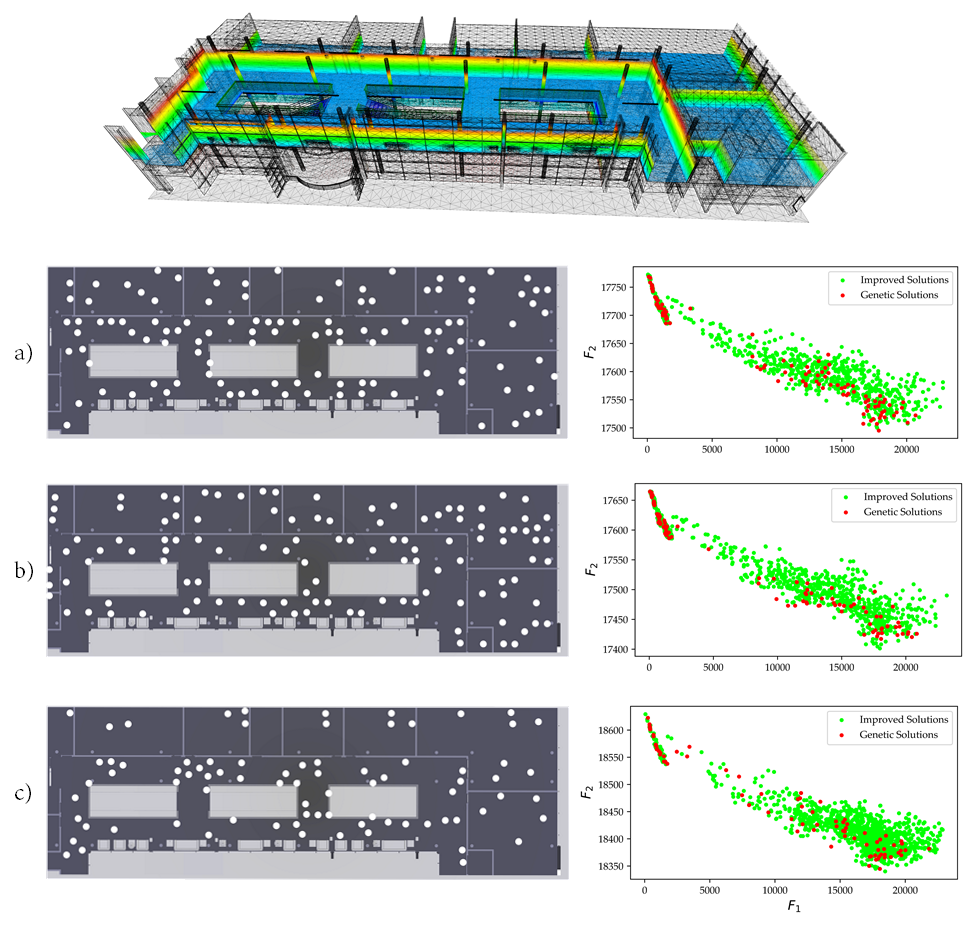
\includegraphics[width=.9\linewidth]{figs/lidar_optimization/ga_results.png}
	\caption{Results obtained by combining local searches and genetic algorithms. The left images depict the final \acrshort{lidar} distribution, whereas the right images show the improvement of intermediate results with regard to the proposed metric ($\textit{Y} \gets$ Minimization, $\textit{X} \gets$ Maximization). a), b) and c) refer to \acrshort{ls} + \acrshort{ga}, \acrshort{sa} + \acrshort{ga} and \acrshort{ts} + \acrshort{ga} combinations. }
	\label{fig:genetic_results}
\end{figure*}

The results from three different pipelines are depicted in Figure \ref{fig:genetic_results}, using a single level of the School scenario. This scenario includes multiple enclosed rooms that cannot be scanned from central areas, as well as gaps in the centre that lead to scanning lower building levels. In this regard, the tabu search (c) obtained a lower number of points, though most of them were gathered in the main room, similar to locally improved solutions being translated to areas with higher geometrical complexity. In contrast to \acrshort{ts}, \acrshort{ls} and \acrshort{sa} provided a higher variety of locations, thereby helping to select a higher number of locations with better coverage of enclosed rooms. Also, note that the \acrshort{lidar} range was limited to $r \gets 5$ \si{\meter} to account for the accuracy loss. Despite \acrshort{ls} and \acrshort{sa} providing similar results, the pipeline \acrshort{sa} + \acrshort{ga} managed to scan the small rooms on the left and right sides due to its wider exploration. Nevertheless, the performance in terms of $F_1$ and $F_2$ was similar for every spatial search, as shown in the scatter plots. It can be concluded that the subsequent \acrshort{ga} is significantly conditioned by the previous local search.

\renewcommand{\arraystretch}{1.15}
\begin{table}
\caption{Configuration of the evaluated genetic algorithm.}
\label{table:genetic_algorithm_parameters}
\begin{tabular}{ll}
\toprule
\textbf{Attributes} & \textbf{Value}\\
\midrule
Maximum number of evaluations & 50,000\\
Population size & 500\\
Number of parents & 250\\
$\mathcal{P}$(Chromosome mutation) & 0.02\\
$\mathcal{P}$(Gen mutation) & 0.1\\
Stagnant population (re-initialization) & 80\%\\
Stuck at local minima (re-initialization) & 30 it. without improving\\
Crossover & Two points\\
Selection & 2-tuple tournament\\
Replacement & Stationary\\
\bottomrule
\end{tabular}
\end{table}
\renewcommand{\arraystretch}{1}

\subsection{Level of overlap}

Previous \acrshort{lidar} locations were improved and narrowed according to $F_1$ and $F_2$ metrics to fit \acrshort{loc}, \acrshort{lod} and \acrshort{loa} requirements. However, \acrshort{loo} was not considered during these optimizations. Instead, it is considered after \acrshort{ga} selection by including new locations aimed at improving the overlapping rather than providing an optimal solution. In this section, several tests were carried out to evaluate the \acrshort{loo} using a greedy approach to 1) sample the scenario and 2) narrow it to a few solutions scattered by controlling the spatial density. Accordingly, Figure \ref{fig:loo_results} shows the initial overlapping as well as the improvement after requiring an overlap of 20\%, 40\% and 60\%. On the right side of the image, the \acrshort{lidar} locations were obtained by limiting the sensor range to 1.5 \si{\meter} and 1 \si{\meter}, respectively. Initial solutions were not improved by means of local searches, thus displaying a grid-like pattern. The last experiment pushes even further the overlapping requirements by scattering solutions with a minimum distance of (6 - $\epsilon$) \si{\meter}. Therefore, the minimum number of solutions to reach one another is 2, though it varies according to their distance. 

\begin{figure*}
    \centering
    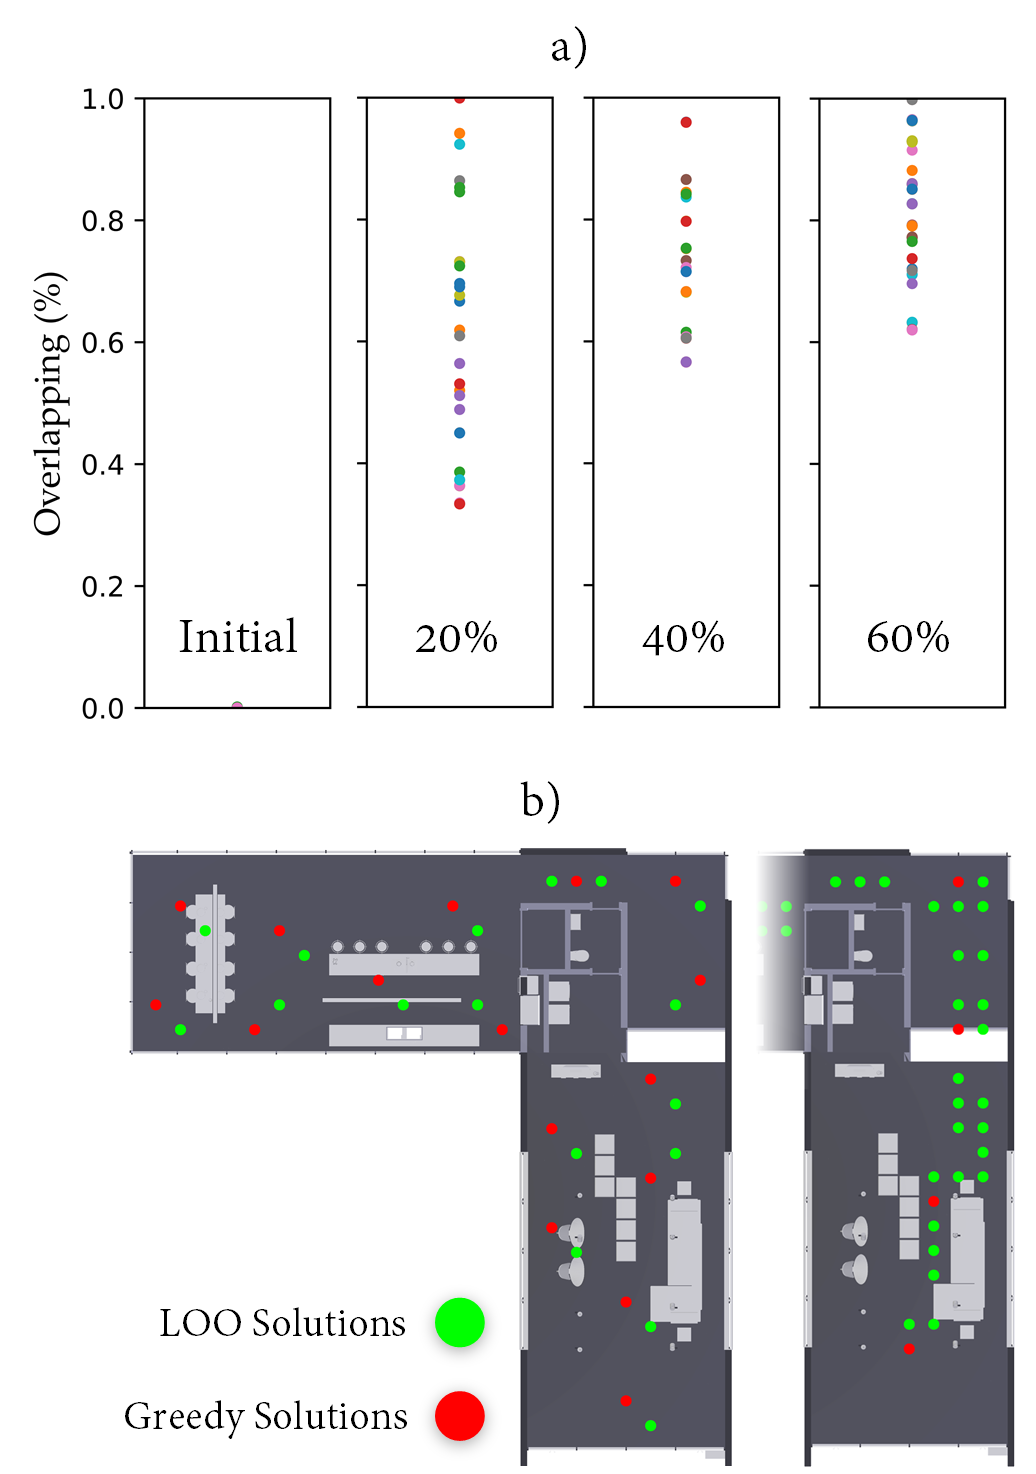
\includegraphics[width=\linewidth]{figs/lidar_optimization/loo_results.png}
	\caption{a) Initial overlap and results obtained after requiring an overlap of 20\%, 40\% and 60\%. b) Rendering of \acrshort{lidar} scans selected by a Greedy approach as well as those selected by the proposed method to enhance the overlap. }
	\label{fig:loo_results}
\end{figure*}

\subsection{Response time}

The main drawback of local searches is the sequential evaluation of \acrshort{lidar} scans. Our proposal is conditioned by \acrshort{gpu}-based \acrshort{lidar} evaluations that cannot be solved in parallel. The performance of the \acrshort{ga} algorithm was improved by solving the whole simulation of a chromosome at once since it is composed of several locations. However, changes in locations must be addressed individually during a local search. On the other hand, improvements based on pre-calculations are more feasible at the expense of higher \acrshort{cpu}-memory usage. Therefore, some optimizations and implementation details are here discussed to provide an efficient solution.

The current \acrshort{ls} approach checks the validity and computes the metric values of every new solution, regardless of the possibility that it may have been previously checked. It seldom occurs with random initialization, though it is more likely to happen with uniformly sampled locations due to the constant step length. Therefore, the response time can be decreased by pre-calculating both the validity and metric results in grid voxels whose length depends on the step length of neighbourhood translations. Still, the latency remains the same for a greedy approach. 

Figure \ref{fig:local_search_response_time} shows the average and global response time for the three \acrshort{ls} approaches. The office building scene was used to conduct this evaluation using the configuration in Table \ref{table:local_search_settings}. The first chart shows the average response time per \acrshort{lidar} location. Hence, latency varies depending on the number of iterations. The global latency comprises the response time from the search and pre-calculation stages. Accordingly, it can be concluded that this approach significantly accelerates the search, except in those algorithms that get easily stuck in local optima or cannot reinitialize. 

\begin{figure*}
    \centering
    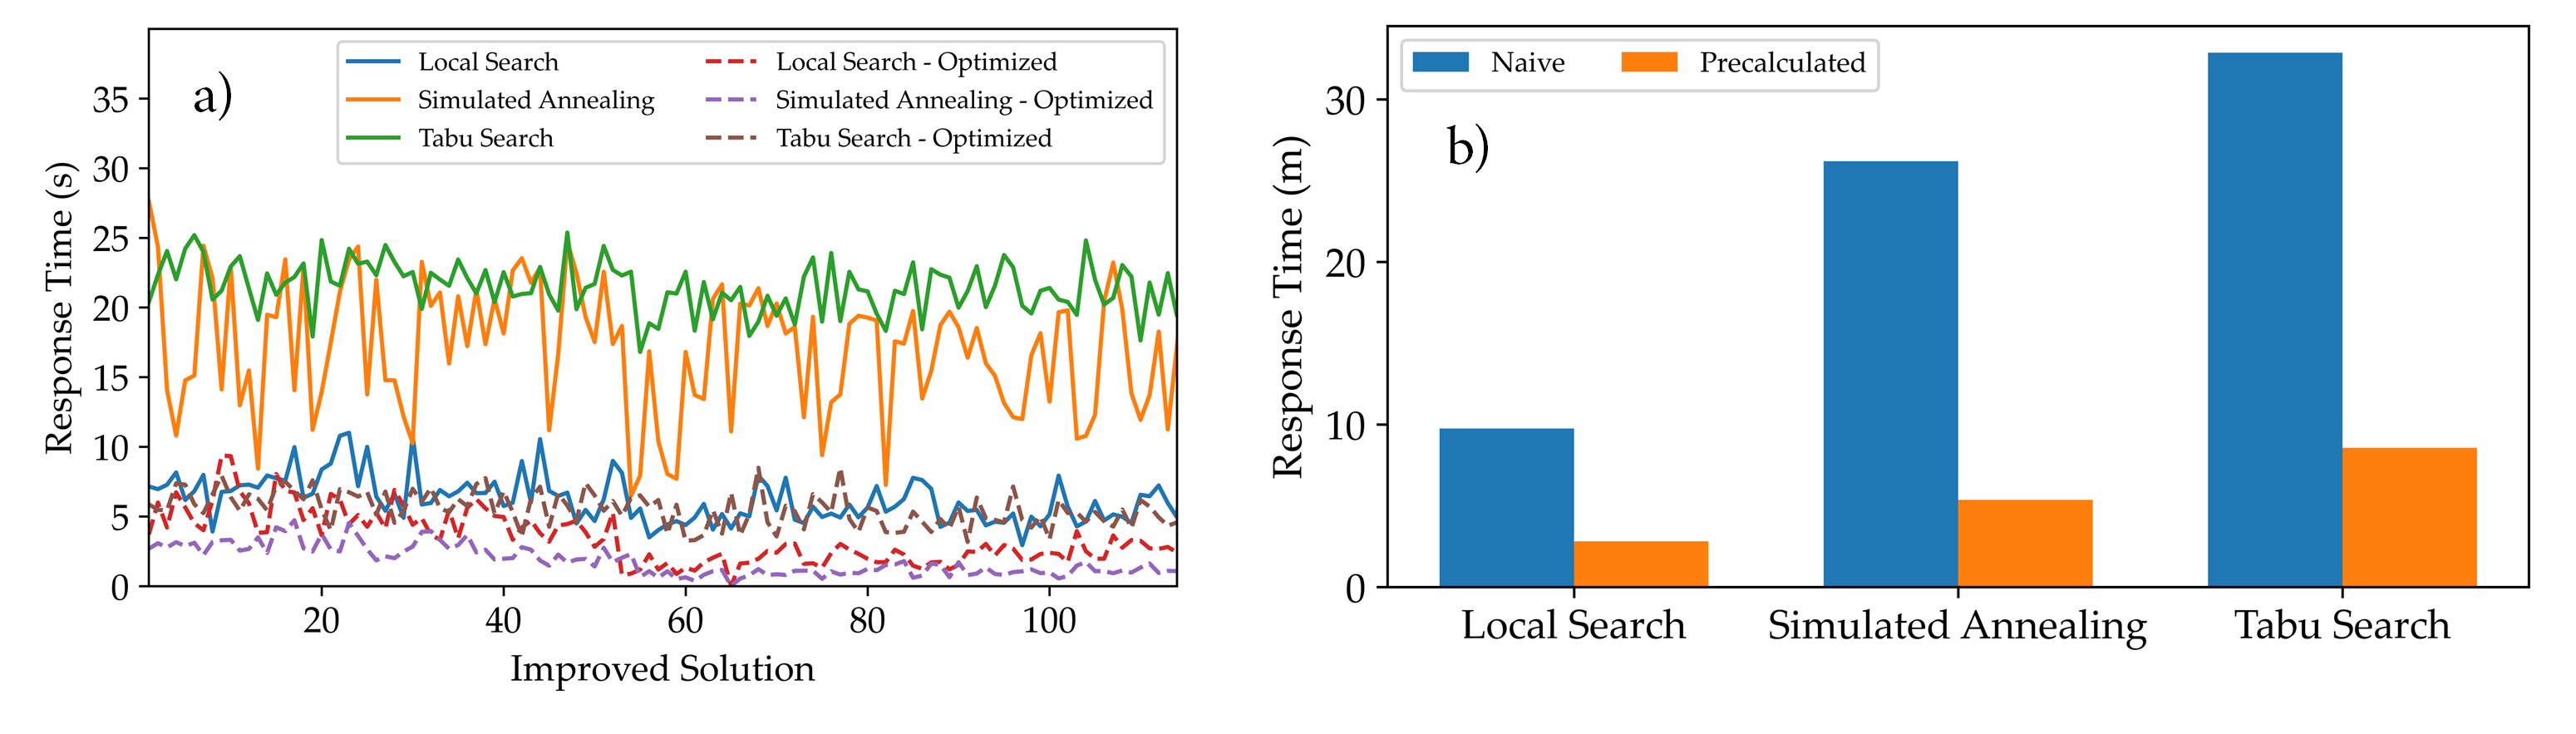
\includegraphics[width=\linewidth]{figs/lidar_optimization/response_time_results.png}
	\caption{a) The average response time per scan for \acrshort{ls} algorithms, implemented by following two approaches: naïve and optimized, and b) summation of response time from previous configurations. }
	\label{fig:local_search_response_time}
\end{figure*}

During the \acrshort{ga}, different chromosomes are evaluated synchronously. Parallelism is, however, possible in other stages: initialization, parent selection, crossover, etc. Hence, it was evaluated whether parallelism was effective enough to get some advantage with the pipeline on the \acrshort{gpu}. Initially, it was implemented as a multi-threading solution on the \acrshort{cpu}. Figure \ref{fig:local_search_response_time} shows that the \acrshort{gpu}-based solution is significantly faster since data is processed in the \acrshort{gpu} for the whole \acrshort{ga} pipeline. Otherwise, data would be transferred to the \acrshort{gpu}, evaluated and subsequently downloaded to the \acrshort{cpu} again (see Figure \ref{fig:ga_response_time}).

\begin{figure}
    \centering
    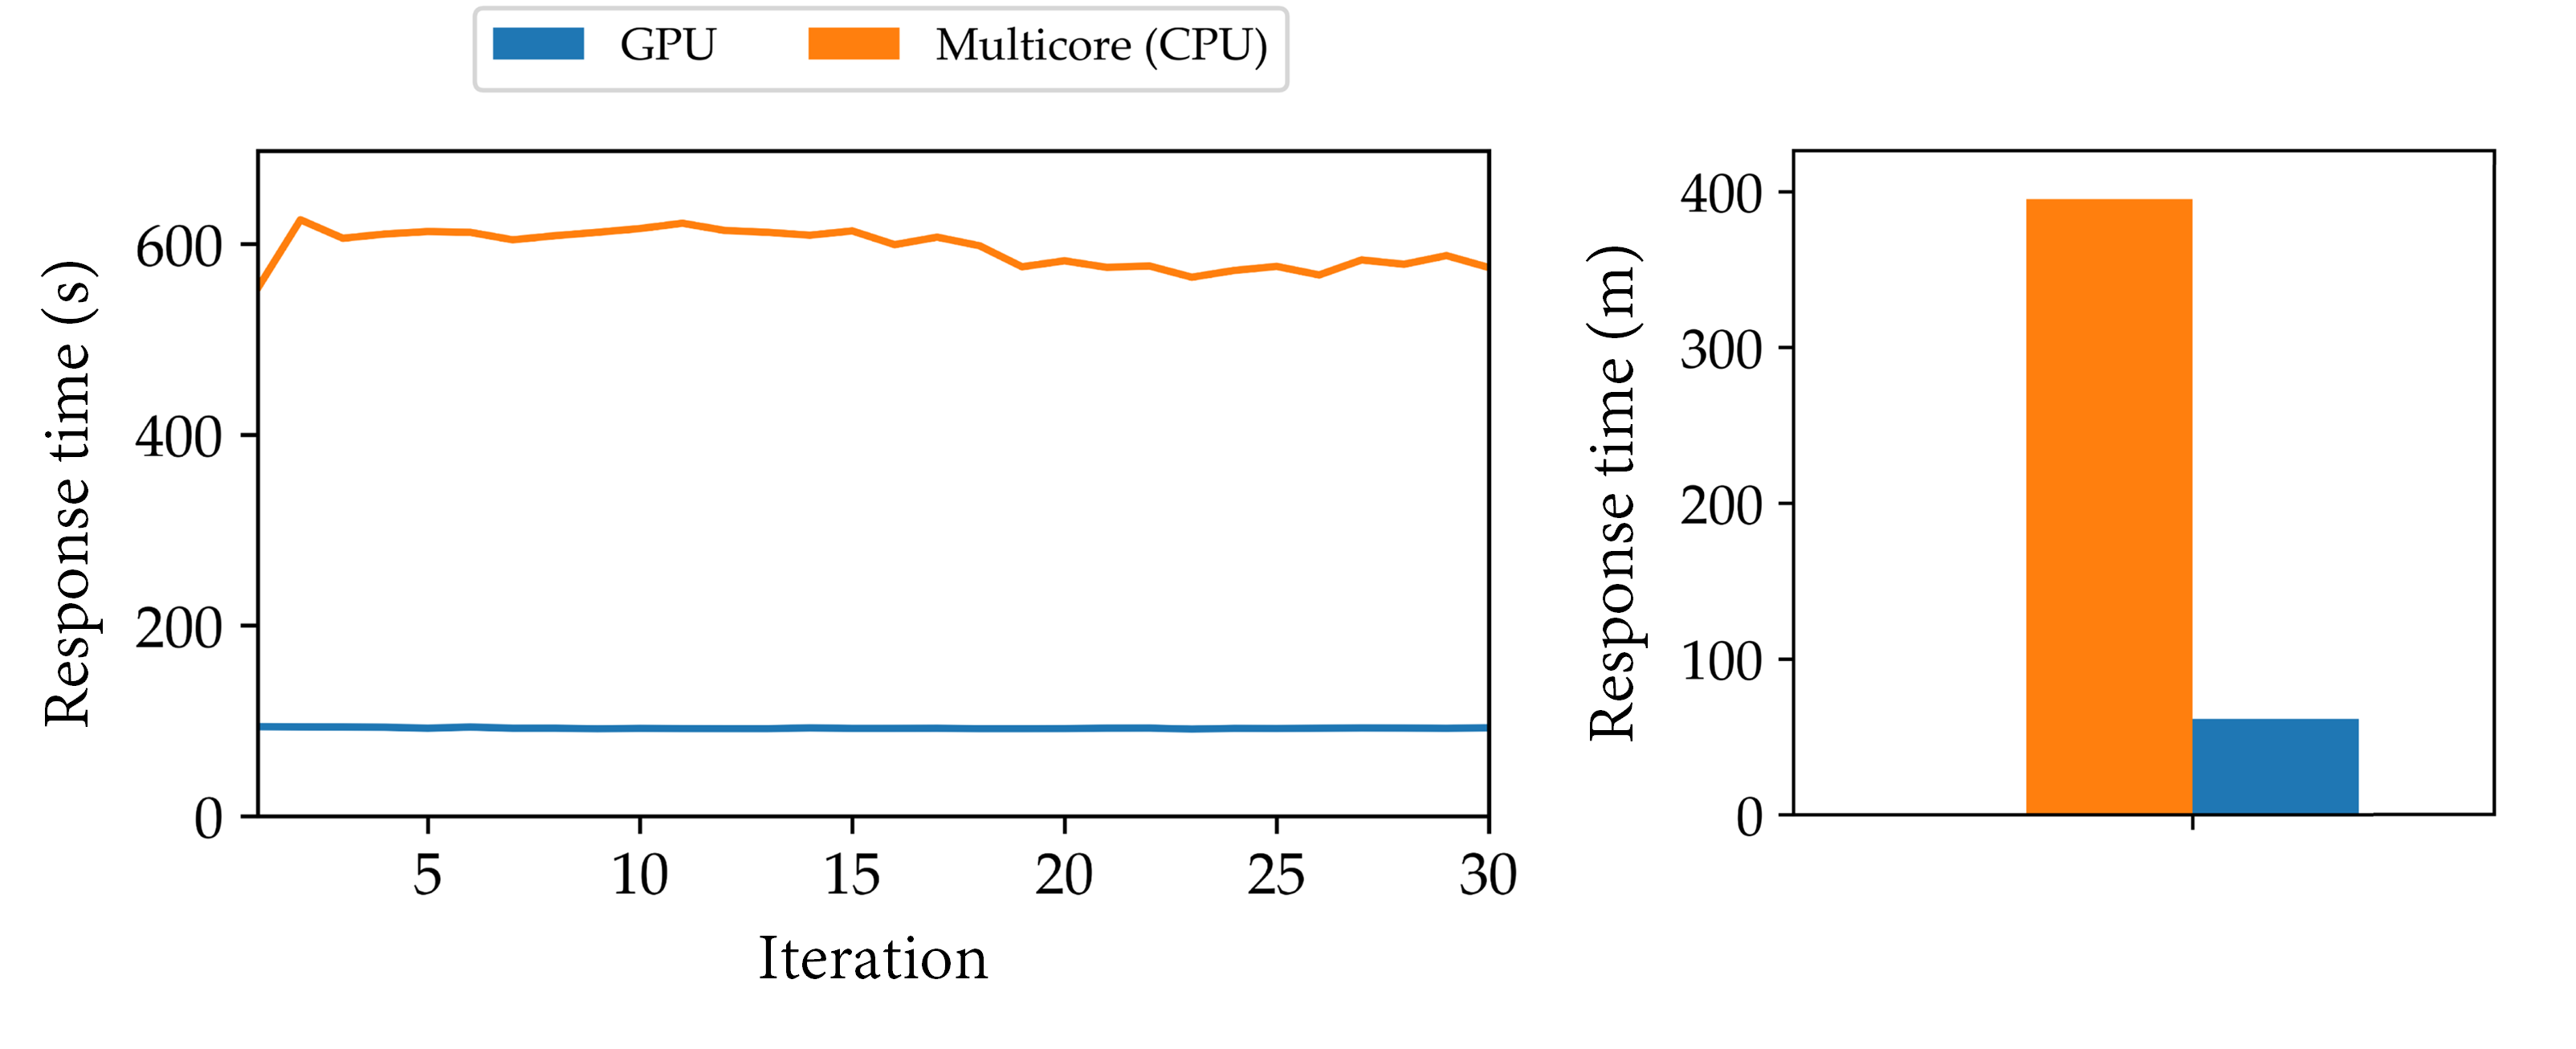
\includegraphics[width=\linewidth]{figs/lidar_optimization/response_time_results_ga.png}
	\caption{Response time of \acrshort{ga}s implemented as \acrshort{cpu} (multi-core) and \acrshort{gpu} solutions. First, the response time is shown per \acrshort{ga} population, and finally, the response time is accumulated for each optimization.}
	\label{fig:ga_response_time}
\end{figure}

\subsection{Variable scan height}

Another contribution of this work is the estimation of the most appropriate scanning height. Figure \ref{fig:cubicle_room} shows the results of $F_1$ and $F_2$ metrics by using 1) fixed height or 2) variable height within the range [1 \si{\meter}, 2 \si{\meter}]. In both cases, the scenario was uniformly subsampled every 0.1 \si{\meter}. The first search was performed over a 2D grid, regardless of being applied over a 3D scene, whereas the second one is 3D. The results are obtained using an experimental environment composed of four outer walls and four inner walls. The latter have gaps placed at different heights, as depicted in Figure \ref{fig:cubicle_room}. The \acrshort{lidar} was first configured as a Velodyne HDL-64E, and then, as a Pandar64 with a wider vertical \acrshort{fov} and non-uniform resolution. Instead of \acrshort{ls}, a Greedy approach was used to evaluate a fine-grained subdivision of the space that is subsequently narrowed to the top-ten locations. As observed in Figure \ref{fig:cubicle_room}, the scans selected by the Greedy approach are placed next to wall holes, thereby allowing to reach more polygons despite being guided by the $F_2$ metric. Therefore, this shows the inclusion of $F_1$ in $F_2$ as well as the capabilities of the proposed pipeline to adapt to different heights.

\begin{figure*}
    \centering
    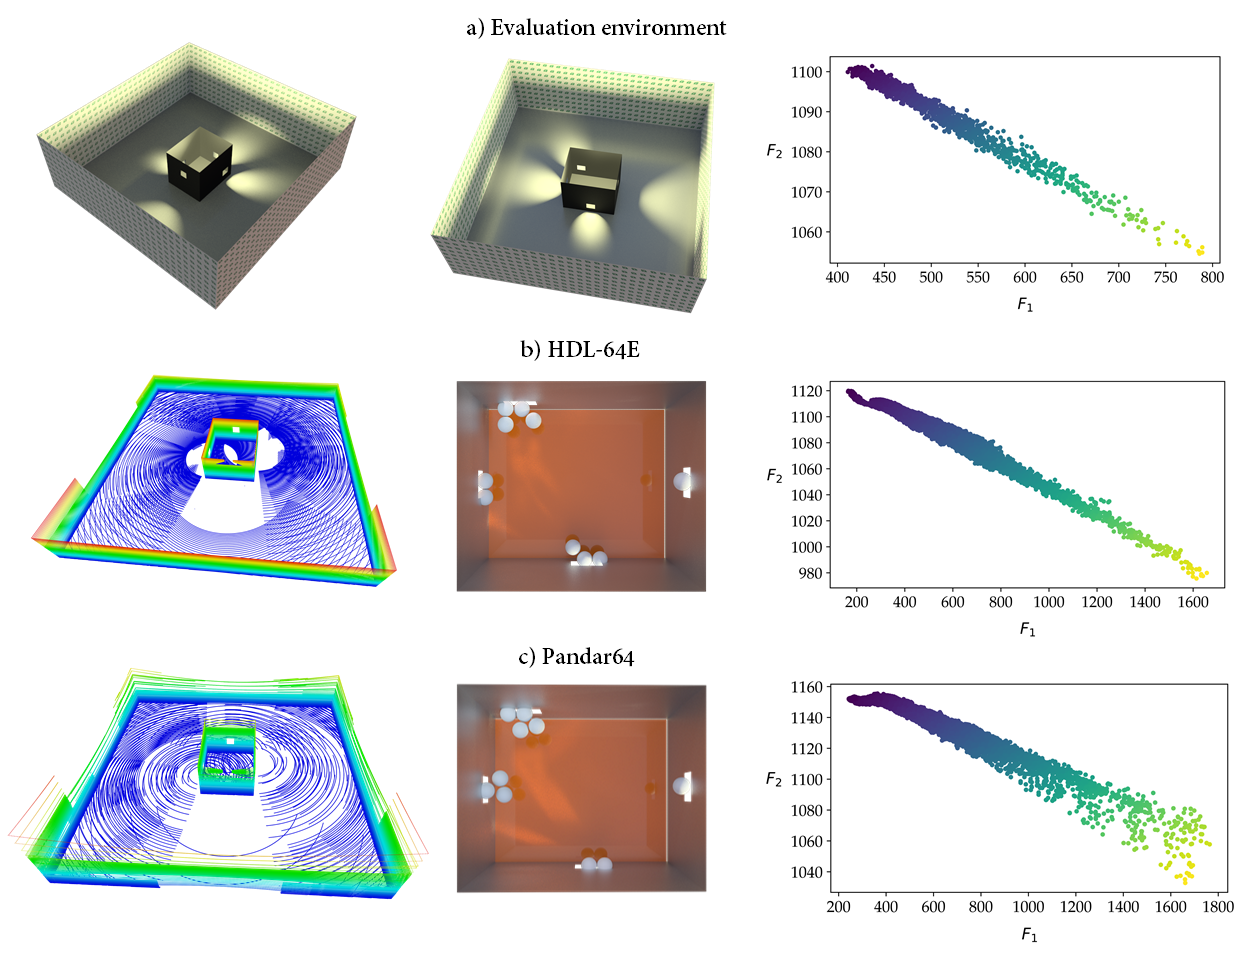
\includegraphics[width=\linewidth]{figs/lidar_optimization/height_variability.png}
	\caption{a) An experimental environment designed for testing the benefits of variable height, and b, c) locations selected by a Greedy algorithm using HDL-64E and Pandar64 \acrshort{lidar} sensors. The scatter plots show the values of $F_1$ and $F_2$ for each initial solution. The first one shows the results of a \acrshort{lidar} with a fixed height. }
	\label{fig:cubicle_room}
\end{figure*}

\section{Conclusions and future work}

In this chapter, a \acrshort{p4s} methodology was described to select the best $n$ scanning locations in complex 3D environments, taking advantage of \acrshort{gpu}-based spatial queries and \acrshort{lidar} scans. Instead of applying a single metaheuristic algorithm, as in most of the revised work, the pipeline was split into two different phases: local optimizations and selection. The proposed metrics do not rely on user-defined values and were implemented as efficient objective functions. Furthermore, some of these metrics, such as the \acrshort{loa}, were improved by considering several criteria (and metrics) at once. Also, the optimal number of required scans is implicitly obtained with a \acrshort{ga} guided by the \acrshort{loc} metric. Finally, algorithms were accelerated with multi-threading in the \acrshort{cpu} and \acrshort{gpu} (the latter only for \acrshort{ga}s). The results showed that the proposed method is capable of constructing a \acrshort{lidar} planning to scan environments with significant occlusion.

Despite being accelerated in \acrshort{cpu} and \acrshort{gpu}, the proposed method is time-consuming due to the dimensionality of the input scenarios and the high resolution of \acrshort{lidar} scans. Therefore, pre-calculating the metric results in uniformly scattered locations ought to be further explored, at the expense of a larger memory footprint. In this regard, compression can also help to reduce the cited footprint by exploring the spatial similarity of close scans. Finally, \acrshort{tls} planning requires discrete locations, whereas other kinds of sensors, such as mobile or aerial scanning, operate with continuous paths.  
